\begin{abstract}
    本文建立了描述信息学比赛的数学模型,基于该模型研究了过往比赛的统计数据,并在此基础上进行推演。本文测量确定了同一名选手的得分波动所服从的分布,基于此从联赛分数推算出了选手整体水平的分布情况,并研究了分级选拔流程的优化方式、回答了有关比赛名次与得分的问题。本文中得到的结论对信息学竞赛流程的优化、选手的日常训练和比赛策略制定具有参考意义。
\end{abstract}

\section{引言}

    中国高中信息学竞赛的参赛人数和竞赛水平在最近十年中快速提高;这种迅猛的发展在让竞赛趋于繁盛的同时,也使得选手和教练对竞赛现状的认知难以跟上节拍。认知的落后引起了一些问题,例如:
    \begin{asparaitem}
        \item {选手对于自己所处的水平段认识不足,从而作出错误的学业规划。}
        \item {出题人对于选手的水平认识不足,导致题目难度和部分分分配失当。}
        \item {选手不了解对手的水平和发挥情况,导致选择了错误的考场策略。}
    \end{asparaitem}

    本文将利用数学工具,基于过往比赛的统计数据来分析信息学竞赛的现状和其中的规律,以为上述问题的解决提供助力。

    \vspace{1.5ex}

    \begin{samepage}
        本文中用到的全部数据和计算程序可以在以下网址下载:\nobreak
        \begin{compactitem}
            \item \inserturl{https://files.cnblogs.com/files/turboboost/qty-thesis-statdata.zip}
            \item \inserturl{https://github.com/TianyiQ/ioi2021-thesis/blob/main/qty-thesis-statdata.zip}
        \end{compactitem}
    \end{samepage}

    \vspace{1.5ex}

    正文分为五个部分:

    \begin{asparaenum}
        \item [\textbf{第二节}]{建立用于描述信息学比赛的数学模型,作为后续分析的基础。}
        \item [\textbf{第三节}]{测量同一名选手的得分波动所服从的分布。}
        \item [\textbf{第四节}]{利用联赛初赛、复赛的得分数据推算出信息学竞赛选手整体水平的分布情况。}
        \item [\textbf{第五节}]{对于在比赛名次中出现的现象进行讨论。}
        \item [\textbf{第六节}]{对于“分级选拔”的选拔方式,提出方法来合理地设置选拔流程。}
    \end{asparaenum}

    由全文的目标决定,本文将不会对初中信息学竞赛进行研究,因此下文中在提到任何比赛时默认指面向高中生的比赛。

\section{建立模型}\label{sec:sec2Modeling}

    \subsection{赛程和赛制}

        在引入模型前,先对信息学竞赛的竞赛流程和比赛形式作简要介绍\footnote{赛程和赛制在近几年有小幅变化,本小节中会尽量兼顾新旧两套机制}。

        信息学竞赛是一系列比赛的统称。这些比赛整体上呈现“逐级递进”的关系,即下一层比赛的优胜者晋级上一层比赛。这些比赛按照级别从低到高,大致排列为\footnote{后文将用下表中的字母标号来代指对应的比赛}:

        \begin{asparaenum}[a.]
            \begin{samepage}
            \item 全国联赛(NOIP/CSP)\ ---\ 初赛
            \nobreak
            \item 全国联赛(NOIP/CSP)\ ---\ 复赛
            \nobreak
            \item 省队选拔赛
            \end{samepage}
            \item 清华/北大学科营(THUWC/PKUWC/THUSC/PKUSC)
            \item 亚太地区竞赛(APIO)
            \item 国家队选拔赛(CTSC/CTS)\ ---\ 非正式选手
            \item 全国冬令营(NOIWC)\ ---\ 非正式选手
            \item 全国决赛(NOI)
            \item 清华/北大集训(CTT)
            \begin{samepage}
            \item 全国冬令营(NOIWC)\ ---\ 正式选手
            \nobreak
            \item 国家队选拔赛(CTSC/CTS)\ ---\ 正式选手
            \nobreak
            \item 国际奥林匹克竞赛(IOI)
            \end{samepage}
        \end{asparaenum}

        \begin{figure}[htbp]
            \centering
            \begin{tikzcd}[column sep=large]
                {} \arrow[r, ">50000"] & a \arrow[d, "20000"]                                     &     \\
                                        & b \arrow[ld, "500"'] \arrow[d, "1000"] \arrow[rd, "500"] &     \\
                d                       & c \arrow[d, "300"] \arrow[l, "300"]                      & efg \\
                                        & h \arrow[d, "70"]                                        &     \\
                                        & ijk \arrow[d, "4"]                                       &     \\
                                        & l                                                        &                 
            \end{tikzcd}
            \caption{信息学比赛间的关系}
            \label{fig:contests}
        \end{figure}

        图\ref{fig:contests}展示了这些比赛间的关系。箭头从低级别比赛指向高级别比赛,表示该低级别比赛的优胜者可以晋级对应的高级别比赛,箭头上标记的数值表示大致晋级人数。

        \vspace{1.5ex}

        赛制即比赛的进行方式和比赛规则。信息学竞赛中采用笔试、COI赛制(机试)、IOI赛制(机试)这三种不同的赛制,表\ref{tab:formats}给出了每种赛制的特点和先前提到的比赛所分别采用的赛制。

        \begin{table}[htbp]
            \centering
            \settabularsize{
            \begin{tabular}{@{}llllll@{}}
                \toprule
                    & 时长                  & 题数                 & 题目类型       & 反馈机制       & 对应比赛   \\ \midrule
                笔试  & 1\textasciitilde 2h & 数十                 & 选择题、填空题     & 无反馈        & a      \\
                COI赛制 & 3\textasciitilde 5h & 3\textasciitilde 4 & 编程题,有多档部分分 & 无反馈        & bcfghk \\
                IOI赛制 & 3\textasciitilde 5h & 3\textasciitilde 4 & 编程题,有多档部分分 & 多次提交、有反馈 & deijl  \\ \bottomrule
            \end{tabular}
            }
            \caption{信息学比赛采用的赛制}
            \label{tab:formats}
        \end{table}

    \subsection{数学模型}

        本小节中将建立用于描述一场信息学比赛的数学模型。

        \subsubsection{基本模型}
        
            为了更清晰地界定模型在现实中的适用范围,需要先明确:现实中怎样的对象能被称为一场“比赛”。

            \begin{definition}[现实比赛]
                一个\textbf{现实比赛},即特定的人群在同样的规则下测试同一套题目的过程。
                一个现实比赛被\emph{参赛人群}、\emph{规则}和\emph{题目}这三个要素所确定。
                \label{def:realContest}
            \end{definition}

            在这一定义下,每年中的 $a\sim l$ 这12个比赛,自然都是现实比赛。而且,不仅是包含两天考试的一场完整的比赛算作现实比赛,单独拿出其中一天也算现实比赛。
            
            \vspace{1.5ex}

            关于“参赛人群”这一概念需要注意两点:
            
            \begin{asparaitem}
                \item 参赛人群只是一个宽泛的范围,而不是具体的选手集合。例如我们可以规定参赛人群为“所有学习信息学的同学”,但这一规定并不关注张三、李四、王五是否是这个人群的成员。这样的规定不会给后续的分析带来不利影响,因为我们只关心关于比赛和人群的统计信息,而不关心每名选手的特点。
                \item 参赛人群不必囊括实际参赛的整个选手群体;例如在NOIP初赛中,“所有报名了初赛的女生”这一参赛群体依然能构成现实比赛。这一点对于后文中跨越不同比赛的分析大有帮助。
            \end{asparaitem}
            
            \vspace{1.5ex}

            接下来定义从现实比赛抽象而来的数学模型。

            \begin{definition}[理想比赛]
                \textbf{理想比赛} $A$ 由二元函数 $\mathcal{H}_A:\left[0,1\right]\times\mathbb{R}\to\mathbb{R}_{\geq 0}$ 确定,其中 $\mathcal{H}_A$ 连续且满足
                \begin{equation}
                    \int\limits_0^1\int\limits_{-\infty}^{+\infty} \mathcal{H}_A(x,\delta)\mathrm{d}\delta\mathrm{d}x=1
                    \label{formula:totalEqual1}
                \end{equation}
                和
                \begin{equation}
                    \int\limits_{-\infty}^{+\infty} \delta\cdot\mathcal{H}_A(x_0,\delta)\mathrm{d}\delta=0,\quad\forall x_0\in\left[0,1\right]
                    \label{formula:expectationEqual0}
                \end{equation}
                此时我们把 $\mathcal{H}_A$ 称为 $A$ 的\textbf{综合分布函数}。
                \label{def:idealContest}
            \end{definition}

            接下来将定义:一个理想比赛何时被认为“描述”了一个现实比赛。这也将同时表明综合分布函数的实际含义。
            
            \vspace{1.5ex}

            首先约定一下记号:

            \begin{asparaitem}
                \item $\mathrm{Pr}\left[A\right]$ 表示事件 $A$ 发生的概率。
                \item $\mathrm{E}\left[X\right]$ 表示随机变量 $X$ 的期望值。
            \end{asparaitem}

            \begin{definition}
                从现实比赛 $B$ 可按如下方式确定一个理想比赛 $A$ :

                \begin{asparaenum}[\bfseries{步骤} 1.]
                    \item 记 $B$ 的参赛选手集合为有限集 $S_B$ ,并在 $B$ 的参赛人群(包括人群内部的具体构成)不变的情况下,假想参赛人数 $\left|S_B\right|$ 趋于无穷。我们之所以能够任意钦定 $\left|S_B\right|$ ,是因为——如先前所述——$B$的定义并未指明具体的选手集合。
                    \item \label{step:realToIdealStep2} 每一名参赛选手 $p$ 在比赛 $B$ 中的实际得分 $\textit{score}_p$ 是一个随机变量,它被各种偶然因素(如临场发挥)所支配,但是它的分布可以由选手 $p$ 和现实比赛 $B$ 的三个要素完全确定。假想对每一名选手 $p$ 计算其期望得分 $\textit{exscore}_p=\mathrm{E}\left[\textit{score}_p\right]$ ,并取所有选手期望得分的最大值,记作 $M_B$ 。由于参赛人数趋于无穷,每一个个人的特征可以忽略,故 $M_B=\max\limits_{p\in S_B} \textit{exscore}_p$ 仅由 $B$ 确定。
                    \item \label{step:realToIdealStep3} 从 $S_B$ 中等概率随机选取一名选手 $p$ ,并:
                    \begin{itemize}[leftmargin=4em]
                        \item 定义取值范围为 $[0,1]$ 的随机变量 $X_B=\frac{\textit{exscore}_p}{M_B}$ 。\footnote{“将每名选手的分数除以最高分数”这一操作,类似于信息学比赛中计算标准分的方式。另外注意到:虽然 $\frac{\textit{exscore}_p}{M_B}\leq 1$ ,但 $\frac{\textit{score}_p}{M_B}$ 可以大于 $1$ }易见随机变量 $X_B$ 的实际取值与考场上的偶然因素无关,而是由选取 $p$ 的方式确定。
                        \item 定义取值范围为 $\mathbb{R}$ 的随机变量 $\Delta_B=\frac{\textit{score}_p-\textit{exscore}_p}{M_B}$ 。易见随机变量 $\Delta_B$ 的实际取值由选取 $p$ 的方式和考场上的偶然因素(如选手临场发挥)共同确定。
                        \item [◦] 请注意,$X_B$ 和 $\Delta_B$ 的定义中所用的 $p$ 是\emph{同一名}随机选择的选手,而不是独立的两次选择。
                    \end{itemize}
                    \item 取 $A$ 的综合分布函数 $\mathcal{H}_A$ 为 $X_B$ 与 $\Delta_B$ 的联合概率密度函数,从而确定 $A$ 。换句话说,对所有 $x_0\in[0,1],\delta_0\in\mathbb{R}$ ,需要满足\footnote{也可以直观地理解为$\mathcal{H}_A(x_0,\delta_0)=\mathrm{Pr}\left[\left(X_B\approx x_0\right)\land\left(\Delta_B\approx\delta_0\right)\right]$,不写作 $X_B=x_0$ 是因为取等概率为 $0$ }
                    \begin{equation}
                        \int\limits_0^{x_0}\int\limits_{-\infty}^{\delta_0} \mathcal{H}_A(x,\delta)\mathrm{d}\delta\mathrm{d}x=\mathrm{Pr}\left[\left(X_B\leq x_0\right)\land\left(\Delta_B\leq\delta_0\right)\right]
                        \label{formula:definitionOfJointDensityFunction}
                    \end{equation}

                \end{asparaenum}

                由\eqref{formula:definitionOfJointDensityFunction}知定义\ref{def:idealContest}的等式\eqref{formula:totalEqual1}满足;由 $\mathrm{E}\left[\Delta_B\right]=0$ 知等式\eqref{formula:expectationEqual0}满足。从而只要联合概率密度函数 $\mathcal{H}_A$ 存在且连续, $A$ 就符合理想比赛的定义。

                对于按上述方式得到的 $A$ ,我们称 $A$ 与 $B$ \textbf{互相对应}。如果按上述过程得到的 $\mathcal{H}_A$ 不连续或根本不存在,则认为不存在与 $B$ 对应的 $A$ 。
                
                \label{def:realIdealCorrespondence}
            \end{definition}

            冗长的定义可以用一句话来作直观的总结:$\mathcal{H}_A\left(x,\delta\right)$ 表示真实水平(即期望得分)约为 $x$ ($x\in\left[0,1\right]$为按最高分折算后的标准分)、实际表现约为 $x+\delta$ (同样表示标准分)的选手的\emph{期望}人数占总人数的比例;之所以实际表现会偏离真实水平——以及这里之所以说“期望人数”——是因为考场上的各种偶然因素为比赛结果带来了随机性。

            可以看到,理想比赛这一模型只考虑了哪些结果\emph{可能}出现,而未考虑哪种结果\emph{实际}出现。而在现实中,能够获知的却只有实际出现的结果——和它恰恰相反。下面定义的概念将处理这一问题。

            \begin{definition}[分数分布函数]
                对理想比赛 $A$ ,定义其\textbf{分数分布函数} $\mathcal{C}_A:\mathbb{R}\to\mathbb{R}_{\geq 0}$ 满足
                $$
                \mathcal{C}_A(s)=\int\limits_{0}^1 \mathcal{H}_A(x,s-x) \mathrm{d}x,\quad\forall s\in\mathbb{R}
                $$

                \label{def:scoreDistribution}
            \end{definition}

            \begin{proposition}[分数分布函数的实际含义]
                对现实比赛 $B$ 和与之对应的理想比赛 $A$ ,假想比赛 $B$ 的参赛人数 $|S_B|$ 趋于无穷,等概率随机选取选手 $p\in S_B$ ,则\footnote{也就是说 $\mathcal{C}_A$ 为随机变量 $\frac{\textit{score}_p}{M_B}$ 的概率密度函数。和先前类似,这里也可以直观理解为 $\mathcal{C}_A(r)=\mathrm{Pr}\left[\frac{\textit{score}_p}{M_B}\approx r\right]$ }:
                $$
                \mathrm{Pr}\left[\frac{\textit{score}_p}{M_B}\leq r\right]=\int\limits_{-\infty}^r \mathcal{C}_A(s)\mathrm{d}s,\quad\forall r\in\mathbb{R}
                $$

                \label{prop:scoreDistributionMeaning}
            \end{proposition}

            \begin{proof}
                \begin{align*}
                    \mathrm{Pr}\left[\frac{\textit{score}_p}{M_B}\leq r\right]
                    &=\mathrm{Pr}\left[X_B+\Delta_B\leq r\right] \\
                    &=\iint\limits_{\left\{(x,\delta):x\in\left[0,1\right],\delta\in\mathbb{R},x+\delta\leq r\right\}}\mathcal{H}_A(x,\delta)\mathrm{d}(x,\delta) \\
                    &=\iint\limits_{\left\{(x,s):x\in\left[0,1\right],s\in\left(-\infty,r\right]\right\}}\mathcal{H}_A(x,s-x)\mathrm{d}(x,s) \\
                    &=\int\limits_{-\infty}^r\left(\int\limits_0^1 \mathcal{H}_A(x,s-x)\mathrm{d}x\right)\mathrm{d}s \\
                    &=\int\limits_{-\infty}^r \mathcal{C}_A(s)\mathrm{d}s
                \end{align*}
            \end{proof}

            在上面四个定义中,涉及到现实情况的部分难免有模糊之处;实际应用中对这几条定义的执行,也不可避免地需要作近似处理。但即便如此,作出这些规定依然能极大地帮助我们厘清思路并发现隐含的前提。

        \subsubsection{特殊情况下的模型}

            在一场现实比赛 $B$ 中,每一个选手 $p\in S_B$ 的实际得分相比真实水平的“得分偏移量” $\frac{\textit{score}_p-\textit{exscore}_p}{M_B}$ 都是一个随机变量。如果所有选手的“得分偏移量”独立同分布,对我们的模型意味着什么?

            容易想到,此时随机变量 $\Delta_B$ 的概率分布就和任何一个选手的“得分偏移量”的概率分布完全相同。换句话说,在定义\ref{def:realIdealCorrespondence}的步骤\ref{step:realToIdealStep3}中,不论我们钦定选取哪一个 $p$ , $\Delta_B$ 取任何一个值的概率都是固定的,且恰好等于在不固定 $p$ 的情况下 $\Delta_B$ 取这个值的概率。再换句话说\footnote{和之前类似,这里之所以不写 $\Delta_B=\delta$ ,是因为取等概率为 $0$ }:$$\mathrm{Pr}\left[(\Delta_B\leq\delta)|(X_B=x)\right]=\mathrm{Pr}\left[\Delta_B\leq\delta\right],\ \forall \left(\delta\in\mathbb{R},x\in\left[0,1\right],\mathrm{Pr}\left[X_B=x\right]>0\right)$$即随机变量 $X_B,\Delta_B$ 独立。在研究这件事之前,我们需要一对新的定义。

            \begin{definition}[期望值分布函数和偏移量分布函数]
                对任意的理想比赛 $A$ :
                \begin{asparaitem}
                    \item 定义其\textbf{期望值分布函数} $\mathcal{X}_A:[0,1]\to\mathbb{R}_{\geq 0}$ 满足 $$\mathcal{X}_A(x_0)=\int\limits_{-\infty}^{+\infty}\mathcal{H}_A(x_0,\delta)\mathrm{d}\delta,\quad\forall x_0\in[0,1]$$
                    \item 定义其\textbf{偏移量分布函数} $\mathcal{D}_A:\mathbb{R}\to\mathbb{R}_{\geq 0}$ 满足 $$\mathcal{D}_A(\delta_0)=\int\limits_0^1\mathcal{H}_A(x,\delta_0)\mathrm{d}x,\quad\forall\delta_0\in\mathbb{R}$$
                \end{asparaitem}
                \label{def:marginalDistributions}
            \end{definition}

            \begin{proposition}[期望值分布函数和偏移量分布函数的实际含义]
                对现实比赛 $B$ 和与之对应的理想比赛 $A$ :
                \begin{asparaitem}
                    \item $\mathcal{X}_A$ 为 $X_B$ 的概率密度函数。换句话说\footnote{也可以直观地理解为:$\mathrm{Pr}[X_B\approx x_0]=\mathcal{X}_A(x_0)$}:$$\mathrm{Pr}[X_B\leq x_0]=\int\limits_0^{x_0} \mathcal{X}_A(x)\mathrm{d}x,\quad\forall x_0\in[0,1]$$
                    \item $\mathcal{D}_A$ 为 $\Delta_B$ 的概率密度函数。换句话说\footnote{也可以直观地理解为:$\mathrm{Pr}[\Delta_B\approx \delta_0]=\mathcal{D}_A(\delta_0)$}:$$\mathrm{Pr}[\Delta_B\leq \delta_0]=\int\limits_{-\infty}^{\delta_0} \mathcal{D}_A(\delta)\mathrm{d}\delta,\quad\forall \delta_0\in\mathbb{R}$$
                \end{asparaitem}
                \label{prop:marginalDistributionsMeaning}
            \end{proposition}

            证明比较显然,这里略去。下面考虑 $X_B,\Delta_B$ 间的独立性带来的性质。

            \begin{proposition}
                对现实比赛 $B$ 和与之对应的理想比赛 $A$ ,如果 $X_B$ 与 $\Delta_B$ 独立,则:
                \begin{equation}
                    \mathcal{H}_A(x_0,\delta_0)=\mathcal{X}_A(x_0)\mathcal{D}_A(\delta_0),\quad\forall (x_0,\delta_0)\in[0,1]\times\mathbb{R}
                    \label{formula:insideImplicationOfIndependence}
                \end{equation}

                更进一步,\eqref{formula:insideImplicationOfIndependence}是 $X_B$ 与$\Delta_B$ 独立的充要条件。

                \label{prop:implicationOfIndependence}
            \end{proposition}

            \begin{proof}
                \begin{align*}
                    &\phantom{\Leftrightarrow\ }\mathrm{Pr}\left[(\Delta_B\leq\delta_0)|(X_B=x_0)\right]=\mathrm{Pr}\left[\Delta_B\leq\delta_0\right],\ \forall \left(\delta_0\in\mathbb{R},\mathrm{Pr}\left[X_B=x_0\right]>0\right) \\
                    &\Leftrightarrow \left(\displaystyle\int\limits_{-\infty}^{\delta_0} \mathcal{H}_A(x_0,\delta)\mathrm{d}\delta\right)\Big/{\mathcal{X}_A(x_0)}=\int\limits_{-\infty}^{\delta_0} \mathcal{D}_A(\delta)\mathrm{d}\delta,\ \forall \left(\delta_0\in\mathbb{R},\mathcal{X}_A(x_0)>0\right)\\
                    &\Leftrightarrow \frac{\mathcal{H}_A(x_0,\delta_0)}{\mathcal{X}_A(x_0)}=\mathcal{D}_A(\delta_0),\ \forall \left(\delta_0\in\mathbb{R},\mathcal{X}_A(x_0)>0\right)\\
                    &\Leftrightarrow \eqref{formula:insideImplicationOfIndependence}
                \end{align*}
                
                最后一步中还需要特别考虑 $\mathcal{X}_A(x_0)=0$ 的情况,不难自行补全。
            \end{proof}

            \begin{definition}[简单理想比赛]
                如果理想比赛 $A$ 满足 \eqref{formula:insideImplicationOfIndependence} 式,则称它是\textbf{简单}的。

                \label{def:simplicityOfContest}
            \end{definition}

            由命题\ref{prop:implicationOfIndependence},对于简单理想比赛 $A$ ,从 $\mathcal{X}_A,\mathcal{D}_A$ 可唯一确定 $\mathcal{H}_A$ ,进而能够确定 $\mathcal{C}_A$ 。

            \begin{proposition}[简单理想比赛的分数分布函数]
                对简单理想比赛 $A$ :
                $$
                \mathcal{C}_A(s)=\int\limits_{0}^1 \mathcal{X}_A(x)\mathcal{D}_A(s-x) \mathrm{d}x,\quad\forall s\in\mathbb{R}
                $$

                \label{prop:scoreDistributionInSimpleContest}
            \end{proposition}

            证明显然,这里略去。

    \subsection{几个关键的假设}\label{sec:keyAssumptions}

        为了使得后续分析成为可能,我们还需要对真实情况作一些近似处理。近似处理的具体方式由本小节的几个假设给出。

        \begin{assumption}
            对任何一个信息学(现实)比赛 $B$ ,都存在符合定义\ref{def:idealContest}的理想比赛 $A$ 与其对应。

            \label{ass:existenceOfIdealContest}
        \end{assumption}

        \begin{assumption}
            对任何一个现实比赛,如果它的\emph{规则}基于COI或IOI赛制,则它对应的理想比赛是简单的。

            \label{ass:simplicityOfCodingContests}
        \end{assumption}

        \begin{assumption}
            考虑所有基于COI或IOI赛制的现实比赛,考察它们对应的理想比赛的偏移量分布,这些分布应该是\emph{相似}的,即它们应该有相同的形式,即使其中的参数可能有不同的取值。

            \label{ass:similarityOfDeltaDistributions}
        \end{assumption}

        在给出下一个假设之前,还需要定义一个概念。

        \begin{definition}[缩放等价]
            对简单理想比赛 $A_1,A_2$ ,当存在线性映射 $f(x)=\alpha x+\beta\quad(\alpha\in\mathbb{R}_{> 0},\beta\in\mathbb{R})$ 同时满足以下条件时,称 $A_1,A_2$ \textbf{缩放等价},称 $f$ 为 $A_1,A_2$ 间的\textbf{等价映射}:
            \begin{asparaenum}
                \item \label{step:equivalenceCondition1} $f(1)=1$
                \item $\mathcal{D}_{A_2}(\alpha\delta)=\mathcal{D}_{A_1}(\delta)\cdot \alpha^{-1},\quad\forall \delta\in\mathbb{R}$
                \item \label{step:equivalenceCondition3} $\widebar{\mathcal{X}}_{A_2}(f(x))=\widebar{\mathcal{X}}_{A_1}(x)\cdot \alpha^{-1},\quad\forall x\in\mathbb{R}$ ,其中
                    $$
                        \widebar{\mathcal{X}}(x)=
                        \begin{cases} 
                            0 & x\notin [0,1] \\
                            \mathcal{X}(x) & x\in[0,1]
                        \end{cases}
                    $$
            \end{asparaenum}

            如果上述映射 $f$ 只满足条件\ref{step:equivalenceCondition1}和\ref{step:equivalenceCondition3},则称 $A_1,A_2$ \textbf{弱缩放等价},称 $f$ 为 $A_1,A_2$ 间的\textbf{弱等价映射}。

            \label{def:equivalenceAfterScaling}
        \end{definition}

        \begin{proposition}[缩放等价的实际含义]
            对缩放等价的 $A_1,A_2$ 及其等价映射 $f$ ,有以下关系\footnote{可以直观理解为:现实比赛 $B_1$ (对应于 $A_1$ )中的分数,经过 $f:x\mapsto\alpha x+\beta$ 的变换之后,变成了现实比赛 $B_2$ (对应于 $A_2$ )中的分数}:
            \begin{asparaenum}
                \item $\displaystyle\int\limits_{-\infty}^{\delta_0} \mathcal{D}_{A_1}(\delta)\mathrm{d}\delta=\displaystyle\int\limits_{-\infty}^{\alpha\delta_0} \mathcal{D}_{A_2}(\delta)\mathrm{d}\delta,\quad\forall\delta\in\mathbb{R}$
                \item $\displaystyle\int\limits_{-\infty}^{x_0} \widebar{\mathcal{X}}_{A_1}(x)\mathrm{d}x=\displaystyle\int\limits_{-\infty}^{f(x_0)} \widebar{\mathcal{X}}_{A_2}(x)\mathrm{d}x,\quad\forall x\in\mathbb{R}$
            \end{asparaenum}

            对于弱缩放等价类似。

            \label{prop:equivalenceAfterScalingMeaning}
        \end{proposition}

        \begin{proof}
            先来看关于 $\mathcal{D}_{A_1},\mathcal{D}_{A_2}$ 的部分:
            \begin{align*}
                \int\limits_{-\infty}^{\delta_0} \mathcal{D}_{A_1}(\delta)\mathrm{d}\delta 
                &=\int\limits_{-\infty}^{\delta_0} \mathcal{D}_{A_2}(\alpha\delta)\alpha\mathrm{d}\delta \\
                &=\int\limits_{-\infty}^{\alpha\delta_0} \mathcal{D}_{A_2}(\alpha\delta)\alpha \mathrm{d}(\alpha\delta)\cdot\alpha^{-1} \\
                &=\int\limits_{-\infty}^{\alpha\delta_0}\mathcal{D}_{A_2}(t)\mathrm{d}t
            \end{align*}

            对于 $\widebar{\mathcal{X}}_{A_1},\widebar{\mathcal{X}}_{A_2}$ 同理,这里不再重复。
        \end{proof}

        \begin{assumption}
            对现实比赛 $B_1$ (对应理想比赛 $A_1$ )和 $B_2$ (对应理想比赛 $A_2$ ),如果
            \begin{asparaenum}
                \item \label{step:equivalenceAssumptionCondition1} $B_1,B_2$ 的\emph{规则}都基于COI或IOI赛制
                \item \label{step:equivalenceAssumptionCondition2} $B_1,B_2$ 的\emph{规则}在除了赛制外的各方面均相同
                \item \label{step:equivalenceAssumptionCondition3} $B_1,B_2$ 的\emph{参赛人群}相同
            \end{asparaenum}

            则 $A_1,A_2$ 一定缩放等价。如果 $B_1,B_2$ 满足条件\ref{step:equivalenceAssumptionCondition1}和\ref{step:equivalenceAssumptionCondition3},则 $A_1,A_2$ 一定弱缩放等价。

            \label{ass:equivalenceBetweenCodingContests}
        \end{assumption}

        对这些假设无法予以严格的证明,但在此可以列举一些感性的理由,来说明它们大体上是可靠的。

        \begin{asparaenum}
            \item \label{step:argumentForAssumptionStep1} 如果假设所有比赛在考查角度上没有差异(因为我们只关心普遍的统计特征,所以这种假设是合理的),那么一名选手的解题能力(即,能够在比赛中解出多大难度的题目)就一定是固定的。
            \item \label{step:argumentForAssumptionStep2} 当组题人为一场比赛选择题目、出题人为命制的题目设置部分分时,他们会有意识地给较难的任务设置较高的分值、给较简单的任务设置较低的分值,而具体多高、多低,则取决于他们心中作的判断。虽然不同的人可能作出不一样的判断,但这些判断应该大体上是“成比例”的。例如:张三认为算法2应当获得三倍于算法1的得分、李四认为算法2应当获得2.5倍于算法1的得分,这两种判断在比例上是大致相符的。
            \item 综合\ref{step:argumentForAssumptionStep1}和\ref{step:argumentForAssumptionStep2},我们知道了:每个选手的能力可以看作是不变的;选手比赛中完成的任务难度与所获分数间的关系,这一关系在不同比赛之间应该是“成比例”的。所以只要选手集合不变,不同比赛的“选手期望得分构成的分布”也应该是“成比例”的(特别地,这两个分布的最大值也应该是相对应的,所以在定义\ref{def:equivalenceAfterScaling}中要求$f(1)=1$)。这就为假设\ref{ass:equivalenceBetweenCodingContests}关于期望值分布的部分和对 $f(1)=1$ 的要求提供了依据。
            \item \label{step:argumentForAssumptionStep4} 根据经验,一名选手考场发挥的稳定与否与水平高低等因素没有明显的相关性;所以虽然不同选手的稳定性存在差异,但是在样本很大时,这种差异不会给统计结果带来较大的系统性的偏差,因此我们近似地认为所有选手\emph{水平发挥}的稳定性是相同的。又因为得分与实际表现出的能力是“成比例”的,所以所有选手\emph{比赛得分}的稳定性也是相同的。这为假设\ref{ass:simplicityOfCodingContests}和假设\ref{ass:similarityOfDeltaDistributions}提供了依据。
            \item 不同的比赛因为比赛天数、试题数目等的不同,可能导致选手得分稳定性的不同(一般来说比赛天数越多,选手得分越稳定)。但如果两场比赛的天数、题数(算作比赛\emph{规则}的一部分)等都相同,就可以用\ref{step:argumentForAssumptionStep4}中的论证,来为假设\ref{ass:equivalenceBetweenCodingContests}关于偏移量分布的部分提供依据。
            \item 真实的比赛中“离散”的特性——比如选择题三分一道——可以在理想化的模型中忽略。这样在人数趋于无穷时,我们很容易想到:其各种统计数据会是“连续”的。因此\ref{ass:existenceOfIdealContest}是一个很自然的假设。
            \item 根据经验,在COI赛制中表现好的选手,在IOI赛制往往表现也很好;反之亦然。因此COI/IOI赛制间的差异至多会对选手期望得分的分布起到缩放的作用,而不会带来本质的改变。类似地,选手在COI/IOI赛制中发挥稳定性的差异,也只有量的差别而无质的差别。所以,认为COI/IOI赛制的比赛有着本质相同(即在缩放后完全相同)的期望值分布、偏移量分布,是合理的。
            \item 假设\ref{ass:simplicityOfCodingContests}会带来一个问题:如果一名选手的期望得分十分接近0,但他的分数波动的幅度仍被认为与其他选手相同,就会使他可能考出“负分数”,并使得分数分布函数在负数处的点值非零。由于本文只研究近似的结果,且考虑到该现象并不会十分显著(因为一场比赛中只会有很少的选手期望得分接近0),所以可以容忍这一不合理的现象。
        \end{asparaenum}

\section{偏移量分布的测量}\label{sec:sec3MeasuringDelta}

    由假设\ref{ass:similarityOfDeltaDistributions},COI/IOI赛制下偏移量分布有一定的形式。本节中,将利用过往比赛的分数数据得到偏移量分布的形式。

    \subsection{数据的获取}

        数据来自以下三场比赛:
        \begin{asparaitem}
            \item 2018年北大集训(字母标号i)
            \item 2019年北大集训(字母标号i)
            \item 2020年北大集训(字母标号i)
        \end{asparaitem}

        选用它们的原因是,北大集训包含连续进行的四场考试,更多的考试场数使得我们能够更精确地估计每一名选手的期望分数。

        这些比赛的参赛情况见表\ref{tab:ctt18to20}。

        \begin{table}[htbp]
            \centering
            \settabularsize{
            \begin{tabular}{@{}lcccc@{}}
            \toprule
             & \multicolumn{1}{l}{参赛总人数} & \multicolumn{1}{l}{正式选手人数} & \multicolumn{1}{l}{非正式选手人数} & \multicolumn{1}{l}{选拔人数} \\ \midrule
            北大集训2018 & 约60 & 50 & 约10 & 15 \\
            北大集训2019 & 约70 & 50 & 约20 & 15 \\
            北大集训2020 & 约90 & 50 & 约40 & 30 \\ \bottomrule
            \end{tabular}
            }
            \caption{三场比赛的参赛情况}
            \label{tab:ctt18to20}
        \end{table}

        根据经验判断,这三场比赛中并非所有选手都全情投入。因此为了保证数据可靠性,对每场比赛只取总排名\footnote{总排名中按每天标准分总和降序排列}中最靠前的 $1.5K\sim 2K$ 名选手的数据,其中 $K$ 表示当场比赛的选拔人数。具体地说:北大集训2018取前30名、北大集训2019取前30名、北大集训2020取前50名。另外为保证比赛之间的统一性,后文中在计算考试分数标准差时,每场比赛只取总排名中前30名的分数。

    \subsection{数据的加工处理}\label{sec:dataPreprocessingOfCTT}

        三场比赛的参赛选手共计110人次,我们将他们视为110名不同的选手。三场比赛共计12场考试,我们将它们视为12个不同的现实比赛。参加这些现实比赛的共计440人次。
        
        虽然这12个现实比赛的参赛人群是相同的(国家集训队选手和精英培训选手),但它们在题目难度等方面并不相同,如果直接将它们的数据汇总起来的话,会使得数据失去意义。为解决这一问题,我们需对比赛得分进行变换。

        \begin{proposition}
            对缩放等价的理想比赛 $A_1,A_2$ 及其等价映射 $f(x)=\alpha x+\beta$\nobreak,有
            $$
            \alpha=\frac{\mathrm{Stddev}\left[\mathcal{C}_{A_2}\right]}{\mathrm{Stddev}\left[\mathcal{C}_{A_1}\right]}
            $$

            其中 $\mathrm{Stddev}\left[F\right]$ 表示以 $F$ 为概率密度函数的随机变量\footnote{换句话说,这样的随机变量 $Y$ 满足 $\mathrm{Pr}\left[Y\leq t\right]=\int\limits_{-\infty}^t F(s)\mathrm{d}s,\quad\forall t\in\mathbb{R}$}的标准差。

            另外注意到由 $f(1)=1$ 可得 $f(x)=1-\alpha(1-x)$ ,所以不必再考虑 $\beta$ 的取值。
            \label{prop:alphaAsQuotientOfStddev}
        \end{proposition}

        \begin{proof}
            \begin{align*}
                \mathcal{C}_{A_1}(s)
                &=\int\limits_0^1 \mathcal{X}_{A_1}(x)\mathcal{D}_{A_1}(s-x) \mathrm{d}x \\
                &=\int\limits_{-\infty}^{+\infty} \widebar{\mathcal{X}}_{A_1}(x)\mathcal{D}_{A_1}(s-x) \mathrm{d}x \\
                &=\int\limits_{-\infty}^{+\infty} \left(\widebar{\mathcal{X}}_{A_2}(\alpha x+\beta)\cdot\alpha\right)\left(\mathcal{D}_{A_2}(\alpha(s-x))\cdot\alpha\right) \mathrm{d}x\\
                &=\int\limits_{-\infty}^{+\infty} \alpha^2\widebar{\mathcal{X}}_{A_2}\left(\alpha x+\beta\right)\mathcal{D}_{A_2}\left(\alpha s+\beta-\left(\alpha x+\beta\right)\right) \mathrm{d}(\alpha x+\beta)\cdot\alpha^{-1}\\
                &=\alpha\int\limits_{-\infty}^{+\infty} \widebar{\mathcal{X}}_{A_2}(t)\mathcal{D}_{A_2}((\alpha s+\beta)-t)\mathrm{d} t\\
                &=\alpha\mathcal{C}_{A_2}(\alpha s+\beta),\quad\forall s\in\mathbb{R}
            \end{align*}

            设连续型随机变量 $Y_1$ 满足其概率密度函数为 $\mathcal{C}_{A_1}$ ,$Y_2$ 满足其概率密度函数为 $\mathcal{C}_{A_1}$ ,则 $\alpha Y_1+\beta$ 与 $Y_2$ 同分布。从而\footnote{这里 $\mathrm{Var}\left[Y\right]$ 表示随机变量 $Y$ 的方差} $\mathrm{Var}\left[Y_2\right]=\mathrm{Var}\left[\alpha Y_1\right]=\alpha^2\cdot\mathrm{Var}\left[Y_1\right]$ ,于是 $\mathrm{Stddev}\left[Y_2\right]=\alpha\cdot\mathrm{Stddev}\left[Y_1\right]$ 。
        \end{proof}

        结合等价映射的实际含义和命题\ref{prop:alphaAsQuotientOfStddev},可以得到对前述12个现实比赛 $B_{1\cdots 12}$ 的分数做变换的方法:
        \begin{asparaenum}[\bfseries{步骤} 1.]
            \item 记 $B_{1\cdots 12}$ 对应的理想比赛为 $A_{1\cdots 12}$ 。
            \item 构造 $A^{\prime}_{1\cdots 12}$ 满足 $A_i$ 与 $A^{\prime}_i$ 缩放等价,且等价映射为 $f_i(x)=1-\frac{1-x}{c\cdot\mathrm{Stddev}\left[\mathcal{C}_{A_i}\right]}$ 。这里 $c=4$ 为根据实际数据所选取的固定常数,用来避免产生负分数。
            \item 则 $A^{\prime}_{1\cdots 12}$ 这12个理想比赛完全相同(即它们的综合分布函数相同),且与 $A_{1\cdots 12}$ 中的每一个缩放等价。
        \end{asparaenum}

        \vspace{1.5ex}

        另外须注意,根据定义\ref{def:realIdealCorrespondence}的步骤\ref{step:realToIdealStep2},我们需要对每个现实比赛 $B_i$ 确定选手期望分数的最大值 $M_{B_i}$ 。这里可以用实际分数的最大值来近似地代替期望分数的最大值。
        
        因为 $A^{\prime}_{1\cdots 12}$ 与 $A_{1\cdots 12}$ 中的每一个缩放等价,所以我们只需测量 $A^{\prime}_{1\cdots 12}$ 的偏移量分布,即可得到结论。现在开始目标将转为测量 $A^{\prime}_{1\cdots 12}$ 的偏移量分布;为便于表述,记 $B^{\prime}_{1\cdots 12}$ 表示 $A^{\prime}_{1\cdots 12}$ 对应的现实比赛。

        现在我们得到了12个完全相同的理想比赛 $A^{\prime}_{1\cdots 12}$ ,和每个理想比赛对应的现实比赛的分数数据;而因为 $A^{\prime}_{1\cdots 12}$ 完全相同,所以所有这些分数数据可以直接合并。现在我们有了一个理想比赛(记为$A^{\prime}$,对应现实比赛 $B^{\prime}$)和对应的440名选手的分数数据。原先的110名选手,每人对应着 $B^{\prime}$ 中的4名选手。

        对于110名选手中的每一位,为了能够对比他在 $B^{\prime}$ 中的期望分数和他的四个“分身”的实际分数,我们还需要估算前者的值。这里可以用该名选手在他所参加的4场现实比赛 $B^{\prime}_i$ 中的平均分,来近似地代替在 $B^{\prime}$ 中的期望分数。

        \vspace{1.5ex}

        综上所述,我们会按如下的流程来加工分数数据:
        \begin{asparaenum}[\bfseries{步骤} 1.]
            \item \label{step:cttDataRefinementStep1} 对12场考试中的每一场,将其中每一名选手的分数除以该场考试的最高分\footnote{即信息学比赛中计算标准分的过程},并以此代替原始分数。
            \item 对12场考试中的每一场,计算总排名前30的选手的分数标准差 $\sigma$ (这里的分数是指步骤\ref{step:cttDataRefinementStep1}中得到的商),然后将其中每个选手的分数 $x$ 施以变换\footnote{除以标准差这一步的作用也可简单理解为,消除题目区分度不同所带来的影响} $x\mapsto 1-\frac{1-x}{4\sigma}$ ,并以此代替原始分数。
            \item 对110名选手中的每一位,计算他在4场考试中的平均分,然后计算他在每场考试中的得分与这一平均分的差。
        \end{asparaenum}

        \vspace{1.5ex}

        这样可以对每名选手计算出4个差值,共计440个值,每个值都表示一名选手在一场比赛中实际得分与期望得分的差距。这440个值即对应着随机变量 $\Delta_{B^{\prime}}$ 的取值,它们将会是下一小节的分析对象。

    \subsection{拟合的方法和结果}

        观察上一小节中获得的440个数值的分布情况,发现:
        \begin{asparaitem}
            \item 整个分布大体上对称,且以$0$为对称中心。
            \item 数值的分布中间稠密、两边稀疏,所有数值的绝对值都小于1。
            \item 分布的形状类似钟形曲线。
        \end{asparaitem}
        
        \vspace{1.5ex}

        受此启发,尝试用正态分布曲线来拟合这些数值。具体方法如下:
        \begin{enumerate}[leftmargin=6em]
            \item [\textbf{步骤 1.}] 对于 $t=-1.0,-0.9,\cdots,1.0$ ,计算:落在 $\left[t-0.05,t+0.05\right)$ 中的数值个数与总个数440的比值。这个比值记作 $c(t)$ 。
            \item [\textbf{步骤 2.}] 在平面直角坐标系中画出 $t-c(t)$ 散点图。
            \item [\textbf{步骤 3.}] 选取合适的参数 $\sigma>0$ ,以使得函数 $$ f(t)=\displaystyle\int\limits_{t-0.05}^{t+0.05} P_{\sigma^2}(x)\mathrm{d} x$$ 的图像与这些 $t-c(t)$ 数据点尽可能贴近(即残差平方和最小)。
        \end{enumerate}

        这里 $P_{\sigma^2}$ 表示期望值为0、方差为 $\sigma^2$ 的正态分布(用 $N(0,\sigma^2)$ 表示)的概率密度函数,满足 $$P_{\sigma^2}(x)=\frac{1}{\sqrt{2\pi}\sigma}\exp{\left(-\frac{x^2}{2\sigma^2}\right)}$$

        再记 $$R_{\sigma^2}(t)=\int\limits_{-\infty}^t P_{\sigma^2}(x)\mathrm{d}x$$ 为正态分布 $N(0,\sigma^2)$ 的累积分布函数,则有\footnote{误差函数 $\mathrm{erf}$ 没有闭合形式,这个式子可以视为$\mathrm{erf}$函数的定义式} $R_{\sigma^2}(t)=\left(1+\mathrm{erf}\left(\frac x{\sqrt{2}\sigma}\right)\right)/2$\nobreak,其中 $\mathrm{erf}$ 表示误差函数。

        最后注意到 $$\int\limits_{t-0.05}^{t+0.05} P_{\sigma^2}(x)\mathrm{d} x=R_{\sigma^2}(t+0.05)-R_{\sigma^2}(t-0.05)$$ 于是在进行拟合的过程中我们可以方便地计算这一定积分。

        \begin{figure}[htbp]
            \centering
            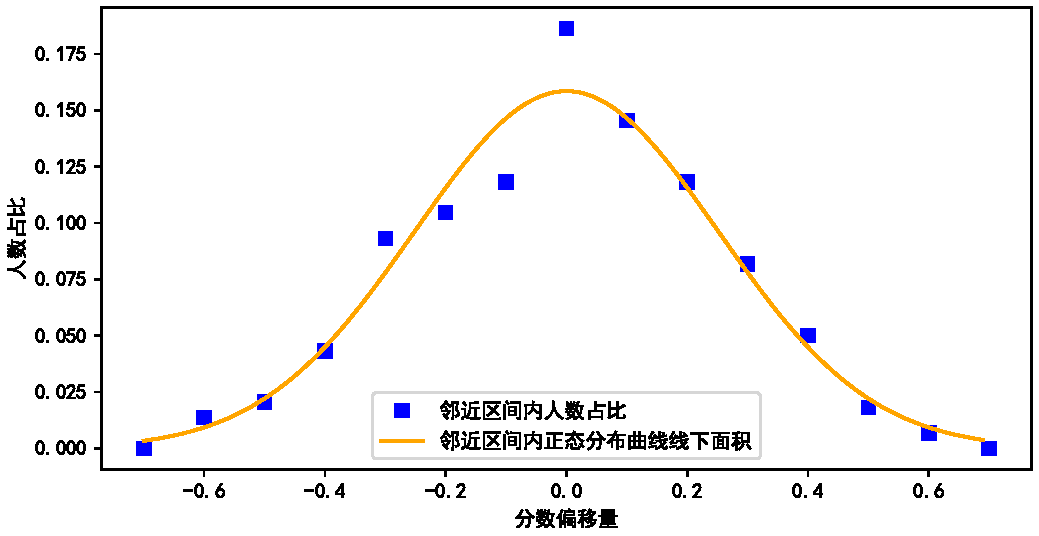
\includegraphics[width=\textwidth]{fig/fittingOffsets.pdf}
            \caption{散点图和拟合结果}
            \label{fig:fittingOffsetsByNormalDistribution}
        \end{figure}

        \vspace{1.5ex}

        图\ref{fig:fittingOffsetsByNormalDistribution}展示了拟合的结果。可以看到,除了约$3$个数据点以外,其余数据点均与曲线贴合紧密。为了验证这些数据是否确实服从正态分布,还需绘制Q-Q图来进行检验。

        \begin{figure}[hp]
            \centering
            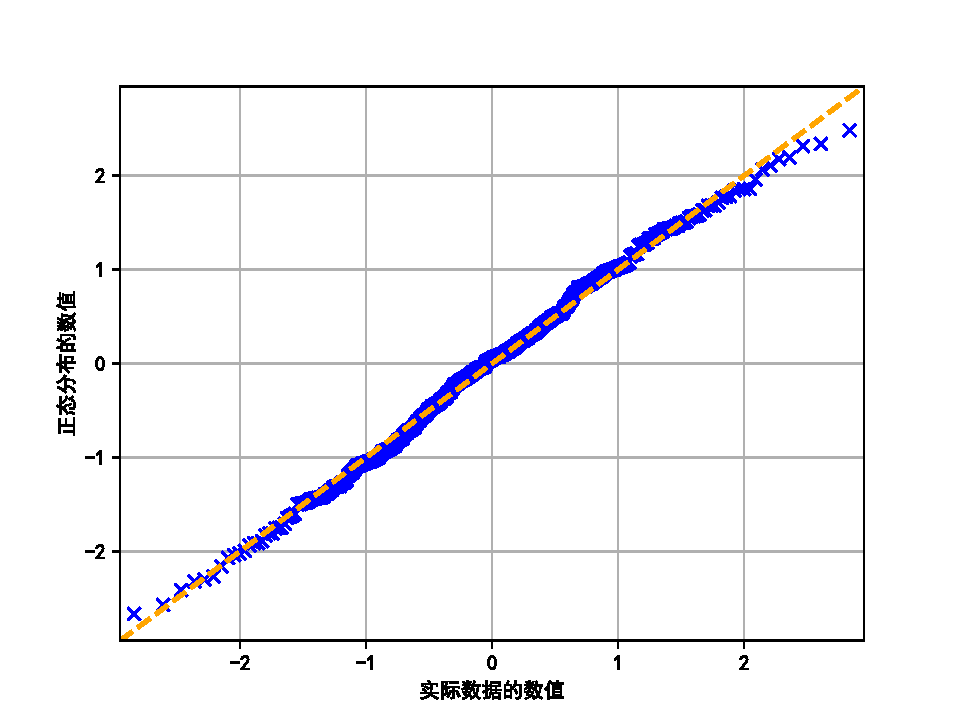
\includegraphics[width=\textwidth]{fig/QQPlot.pdf}
            \caption{Q-Q图,关于比赛分数差值数据和正态分布绘制}
            \label{fig:QQPlot}
        \end{figure}

        \vspace{1.5ex}

        图\ref{fig:QQPlot}展示了所绘制的Q-Q图。注意,该图的坐标轴经过缩放,故坐标轴上标注的数值仅能代表相对的比例关系。
        
        图\ref{fig:QQPlot}中有440个蓝色叉号,所有叉号的横坐标、纵坐标非严格递增。其中第 $k$ 个叉号($1\leq k\leq 440$)对应着440个数值中的第 $k$ 小值 $\textit{val}_k$ ,叉号的横坐标 $x_k$ 等于对应的数值 $\textit{val}_k$ ,而叉号的纵坐标 $y_k$ 等于:440个服从正态分布 $N(0,\sigma^2)$ 的数值中,第 $k$ 小值的期望;其中的 $\sigma$ 是待定的参数。可以证明 $y_k$ 满足 $R_{\sigma^2}(y_k)=\frac {k}{440+1}$ ,于是由这一关系可以求出 $y_k$ 。

        如果这440个数值服从 $N(0,\sigma^2)$ 的话,容易想到应该有 $x_k\approx y_k$ ,也就是说所有叉号落在直线 $y=x$ 附近。我们通过选取合适的 $\sigma>0$ 来让叉号尽可能贴近直线 $y=x$ ,最终的结果就是图\ref{fig:QQPlot}。可以看到,叉号与直线紧密贴合,所以这些数据确实服从正态分布\footnote{注意到,缩放坐标轴和改变 $\sigma$ 的取值,这两种操作对图像的改变其实是完全相同的,所以缩放坐标轴不会影响结论的可靠性}。又由假设\ref{ass:similarityOfDeltaDistributions},这一规律对任何COI/IOI赛制的比赛都成立。

        \begin{theorem}[偏移量分布的形式]
            对任何基于COI或IOI赛制的现实比赛,其对应的理想比赛的偏移量分布是期望值为$0$的正态分布。
            \label{thm:normalityOfOffsetsDistribution}
        \end{theorem}

\section{选手整体水平的估计}\label{sec:estimationOfOverallDistribution}

    本节将借助联赛初赛(字母标号a)和联赛复赛(字母标号b)的分数数据,来估计全国信息学竞赛选手整体水平的分布情况。

    选手的“水平”是一个模糊的概念;为了将其量化,我们将用一名选手在联赛复赛中的期望分数来衡量这名选手的水平。

    虽然由假设\ref{ass:equivalenceBetweenCodingContests},不同年份的联赛复赛(所对应的理想比赛)是缩放等价的;但它们毕竟不相同,因此“在联赛复赛中的期望分数”这一概念需要澄清。\ref{sec:dataPreprocessingOfNOIP}小节将处理这一问题,并完成对复赛分数数据的初步分析。接着,\ref{sec:analysisOfBothRounds}小节将从分数数据中,得到复赛在去除了初赛的筛选所带来的影响后,其(对应的理想比赛的)分数分布函数的表达式。最后,\ref{sec:calculatingXofSecondRound}小节将从分数分布计算出对应的期望值分布,这一分布即可体现全国选手整体水平的分布情况。

    本节中会多次对现实情况作近似、作假设,于是也会不可避免地带来可观的误差。因此,本节的目标旨在估计而非精准计算,所得的结果仅能反映趋势而不保证精确。

    \subsection{复赛分数数据的获取、加工和拟合}\label{sec:dataPreprocessingOfNOIP}

        数据来自以下4场比赛:
        \begin{asparaitem}
            \item NOIP2016\ ---\ 复赛(字母标号b)
            \item NOIP2017\ ---\ 复赛(字母标号b)
            \item NOIP2018\ ---\ 复赛(字母标号b)
            \item CSP2019\ ---\ 复赛(字母标号b)
        \end{asparaitem}

        \vspace{1.5ex}

        之所以只采用2016年到2019年的比赛,是出于三个原因:
        \begin{asparaitem}
            \item 年代过于久远的比赛对当今的参考意义有限。
            \item 仅有的数据来源为NOI官网上的获奖名单公示,故只能取得获奖选手的分数信息。而自2016年起CCF更改了获奖规则,增加了获奖人数,使得可以获取的数据量大了许多。
            \item 2020年的比赛规则有所更改(两天六题改为一天四题),所以假设\ref{ass:equivalenceBetweenCodingContests}不再能保证2020年复赛与其他年份复赛缩放等价。
        \end{asparaitem}

        \vspace{1.5ex}

        \begin{table}[htbp]
            \centering
            \settabularsize{
            \begin{tabular}{@{}lccccc@{}}
                \toprule
                    & \multicolumn{1}{l}{参赛人数} & \multicolumn{1}{l}{获奖人数} & \multicolumn{1}{l}{满分} & \multicolumn{1}{l}{最高分} & \multicolumn{1}{l}{获奖分数线} \\ \midrule
                NOIP2016复赛 & 约8300  & 约5900  & 600 & 600 & 100 \\
                NOIP2017复赛 & 约10300 & 约6600  & 600 & 600 & 80  \\
                NOIP2018复赛 & 约12900 & 约8000  & 600 & 600 & 120 \\
                CSP2019复赛  & 约13900 & 约8800  & 600 & 600 & 80  \\ 
                总计         & 约45400 & 约29300 &     &     &     \\ \bottomrule
            \end{tabular}
            }
            \caption{4场比赛的相关数据}
            \label{tab:noip16to19}
        \end{table}

        表\ref{tab:noip16to19}展示了关于这4场比赛的几项统计数据。

        \vspace{1.5ex}

        由假设\ref{ass:equivalenceBetweenCodingContests},这4场现实比赛(所对应的理想比赛)是缩放等价的。进而由命题\ref{prop:alphaAsQuotientOfStddev},这4场现实比赛所对应的理想比赛,在对分数作变换(变换方式见\ref{sec:dataPreprocessingOfCTT}小节)后,将成为完全相同的理想比赛。

        于是,与\ref{sec:dataPreprocessingOfCTT}小节类似,数据加工将按以下步骤进行:
        \begin{asparaenum}[\bfseries{步骤} 1.]
            \item 将所有比赛中所有选手的分数除以当场比赛的最高分(也就是计算标准分;注意到最高分等于满分),用以代替原始分数。
            \item \label{step:noipDataRefinementStep2} 去除所有$<0.2$的分数。这是因为在这4场比赛中,获奖分数线与最高分的商的最大值为$0.2$;这意味着分数低于$0.2$的选手中有一部分未能获奖,于是这些选手中其余部分的数据也失去意义,因此一并剔除。
            \item 对每场比赛计算分数标准差 $\sigma$ ,然后对分数作变换 $R:x\mapsto 1-\frac{1-x}{5.52\sigma}$ ,并用变换结果代替原分数。使用系数$5.52$的理由稍后说明。
            \item 对每场比赛计算最低分,取所得的4个最低分的最大值$T$,并剔除所有$<T$的分数。这一步的理由与步骤\ref{step:noipDataRefinementStep2}中的类似:分数低于$T$的部分选手未能获奖,故将这些选手连同已获奖的那些一并剔除。计算可得 $T\approx 0.200$ ,与步骤\ref{step:noipDataRefinementStep2}中的阈值保持一致;这正是系数$5.52$的主要作用。
            \item 现在所有这些分数数据属于同一理想比赛 $A$ (满足 $A$ 与原先4个现实比赛所对应的理想比赛缩放等价),将它们汇集起来即可。注意到我们所取得的并非完整的分数数据,而只是$\geq 0.2$的那一部分分数。
        \end{asparaenum}

        \vspace{1.5ex}

        本节中我们约定使用理想比赛 $A$ 作为衡量选手水平的标尺,也就是说我们将用一名选手在 $A$ 中的期望分数,来代表该名选手的水平。后文中如果作为一个现实比赛提到“联赛复赛”,则默认指 $A$ 对应的现实比赛。

        \vspace{1.5ex}

        经过上述加工后,我们得到了22093个落在$[0.2,1]$之中的分数数据。由命题\ref{prop:scoreDistributionMeaning},这些数据应当服从 $\mathcal{C}_A$ 所描述的概率分布。
        
        接下来我们将确定函数 $\mathcal{C}_A:\left(0,1\right)\to\mathbb{R}_{\geq 0}$ ,满足在任何一个区间 $\left(a,b\right)$ 上,$\mathcal{C}_A$ 的定积分在数值上约等于:分数落在$\left(a,b\right)$中的选手人数,与总人数45400的比值。
        
        在对十余种常见函数和常见概率分布进行拟合之后,我们发现对数函数 $f(s)=-\log(s)$ 满足前述要求,且与已获得数据的贴合程度大幅好于所尝试的其他函数。此外,不难验证对数函数 $f(s)=-\log(s)$ 在 $(0,1)$ 上非负且定积分等于 $1$ ,因此是一个合法的分数分布函数。以下将在实际数据和据对数函数计算出的数值之间进行比对,并展示结果。

        \begin{enumerate}[leftmargin=6em]
            \item [\textbf{步骤 1.}] \label{step:plottingNoipStep1} 对于 $t=0.25,0.35,\cdots,0.95$ ,计算:落在 $\left[t-0.05,t+0.05\right]$ 中的分数个数与总人数45400的比值。这个比值记为 $c(t)$ 。
            \item [\textbf{步骤 2.}] 关于 $<0.2$ 的分数段,我们不了解其中具体的分数分布,只知道这一部分共有$45400-22093=23307$人,占比 $\frac{23307}{45400}\approx 0.513$ 。为了与步骤\ref{step:plottingNoipStep1}中的数据统一,我们将数值$0.513$乘以$$\frac{\int_{0.05}^{0.15}-\log(s)\mathrm{d}s}{\int_{0}^{0.2}-\log(s)\mathrm{d}s}$$以将其换算为分数段 $(0.05,0.15)$ 上的人数占比,并记作 $c(0.1)$ 。
            \item [\textbf{步骤 3.}] 在平面直角坐标系中画出 $t-c(t)$ 散点图。
            \item [\textbf{步骤 4.}] 检查函数 $$f(t)=\int\limits_{t-0.05}^{t+0.05}-\log(x)\mathrm{d}x$$ 的图像是否与 $t-c(t)$ 散点图吻合。
        \end{enumerate}

        \begin{figure}[htbp]
            \centering
            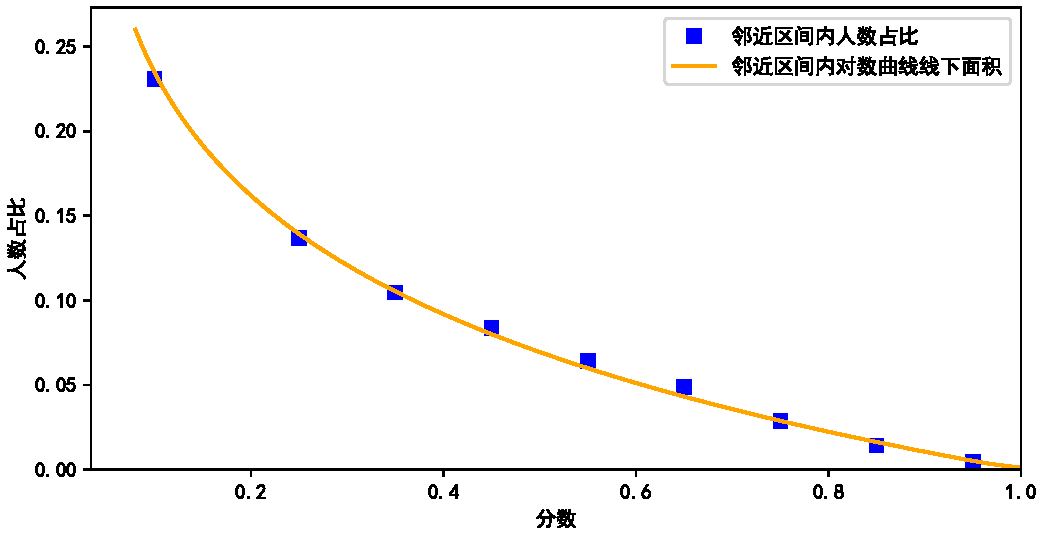
\includegraphics[width=\textwidth]{fig/fittingNoipScores.pdf}
            \caption{散点图和拟合结果}
            \label{fig:fittingNoipScoresByLogCurve}
        \end{figure}

        图\ref{fig:fittingNoipScoresByLogCurve}展示了比对的结果。可以看到全部数据点与曲线贴合紧密,且算得残差平方和约为$9.2\cdot 10^{-5}$,显示出了较好的拟合效果。基于此,我们确定取 $\mathcal{C}_A(s)=-\log(s)$ 。

        \begin{proposition}
            $\mathcal{C}_A(s)=-\log(s)$ ,其中 $s\in(0,1]$ 且 $A$ 是根据\ref{sec:dataPreprocessingOfNOIP}小节中描述的过程所确定的理想比赛。
            \label{prop:scoreDistributionOfStandardizedNoip}
        \end{proposition}
            
    \subsection{结合初赛的分析}\label{sec:analysisOfBothRounds}

        这一小节将对于复赛所对应的理想比赛 $A$ ,在去除了初赛的筛选性所带来的影响后,计算所得的新的理想比赛(记为 $A^\prime$ )的分数分布函数。其中,\ref{sec:dataOfPreliminaryRound}小节将给出初赛分数数据的来源,\ref{sec:assumptionsOnPreliminaryRound}小节将结合这些数据给出关于初赛的几个假设;第\ref{sec:estimationOfOverallDistribution}节的其余部分都将依赖于这些假设。\ref{sec:parameterOfDeltaDistribution}小节将计算初复赛(所对应理想比赛)的偏移量分布的标准差,以为\ref{sec:counteringPreliminaryRound}小节中 $\mathcal{C}_{A^\prime}$ 的计算做好准备。

        \subsubsection{初赛分数数据的获取}\label{sec:dataOfPreliminaryRound}

            分数数据采用NOIP2018初赛北京赛区的成绩。该场比赛共781人获得非零分数(零分视为缺考),其中536人晋级复赛并获得非零分数;该场比赛满分100分,最高分96分,晋级分数线约为35分;全国最高分为100分。有关初赛的全部数据获取自官方网站上的成绩公示。

            采用该场比赛的原因:后续分析需要分数表上包含选手姓名;而笔者所能找到的其他年份、其他省市的成绩公示,均未包含这一信息。

            知道了选手姓名,我们就可以查询该名选手在NOIP2018复赛中的得分。通过这种方式,我们获得了536名晋级者的初赛和复赛分数。由于官方网站上的成绩公示仅包括获奖选手,这里所使用的北京选手复赛分数是按民间数据测试出的成绩。

            \vspace{1.5ex}

            除此以外,在\ref{sec:counteringPreliminaryRound}小节中,还将使用CSP2019初赛的全国分数数据,这些数据从官方网站上各省市发布的成绩公示汇总得到。CSP2019初赛报名人数48812人,由于个别省份仅公示了晋级选手或未缺考选手的分数,最终收集到47264人的数据。

            全国分数数据的来源之所以采用CSP2019,是因为自2019年起才有完整的初赛分数公示。

        \subsubsection{关于初赛的几个假设}\label{sec:assumptionsOnPreliminaryRound}

            不同于复赛,信息学联赛的初赛是分省考试、分省排名的,这会给本文的分析带来很大困难。为了规避这一问题,我们作如下假设:

            \begin{assumption}
                每一年的联赛初赛为全国统一考试、统一排名,全国范围内分数最高的若干名选手晋级复赛。

                \label{ass:preliminaryRoundsOfAllProvincesUnite}
            \end{assumption}

            作出这一假设,意味着忽略不同省市间选手水平和竞争激烈程度上的差异,并用全国整体的选手水平和竞争激烈程度来代替之。即使如此,我们一般也并不能直接用一个地区的数据来“代表”全国的数据,而是只有在所研究的量与地域没有明显关联时(例如\ref{sec:parameterOfDeltaDistribution}小节中研究同一名选手的初赛得分与复赛得分间的关系)才能这样做。

            \vspace{1.5ex}

            在给出下一个假设前,先对2018北京初赛的分数做一点分析。

            \begin{asparaenum}[\bfseries{步骤} 1.]
                \item 将536名晋级选手按初赛分数分组:分数在$[30,40)$中的、在$[40,50)$中的、……、在$[90,100)$中的,分别分为一组,共计7组。
                \item 对每一组计算初赛平均分和复赛平均分。
                \item 对每一组,以复赛平均分为横坐标、初赛平均分为纵坐标,将数据点画在二维平面上,并将这些数据点连成折线图。
            \end{asparaenum}

            \begin{figure}[htbp]
                \centering
                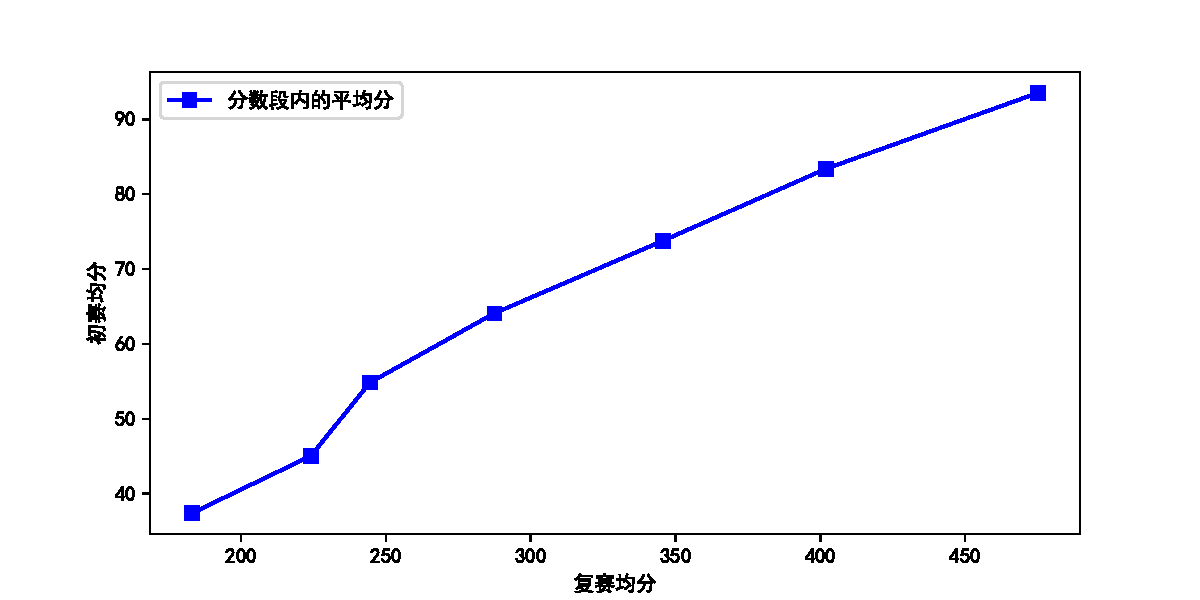
\includegraphics[width=\textwidth]{fig/plottingAvgScores.pdf}
                \caption{平均分折线图}
                \label{fig:plottingAvgScores}
            \end{figure}

            所得的折线图如图\ref{fig:plottingAvgScores}所示。可以看到,这些数据点近似地连成一条直线;这提示我们,初赛分数与复赛分数之间存在一个线性的对应关系。
            
            基于这一观察,我们作出如下假设:

            \begin{assumption}
                记现实比赛 $B_1$ 为联赛初赛,\textbf{取参赛人群为实际晋级复赛的全体选手};记现实比赛 $B_2$ 为联赛复赛;则 $B_1,B_2$ 对应的理想比赛缩放等价。

                \label{ass:equivalenceBetweenTwoRounds}
            \end{assumption}

            注意:“取参赛人群为实际晋级复赛的全体选手”这一规定,只限制了参赛人群,而并未要求这些选手在理想比赛中的分数也一定得达到晋级的标准。也就是说,虽然我们只取那些在现实中达到了晋级分数线的选手,但在构造对应的理想比赛时,我们忽略现实中发生了什么,仍然只考察每名选手分数波动的概率分布和他的期望分数。

            \vspace{1.5ex}

            关于这一假设需要作几点说明:
            \begin{asparaenum}
                \item \ref{sec:keyAssumptions}小节中,我们在为假设\ref{ass:equivalenceBetweenCodingContests}予以辩护时,断言了“一名选手的水平是固定的,不会随比赛的改变而改变”。但是,由于考察内容的不同,一名选手在 $B_1$ 和 $B_2$ 中的能力差异可能较大,故上述断言在将初赛(即 $B_1$ )加入考虑范围后似乎不再成立。
                \item \label{step:argumentForAssumptionOnPreliminaryRoundStep2} 为了使前述断言仍然成立,在\ref{sec:analysisOfBothRounds}小节内,我们需暂时改变命题\ref{def:realIdealCorrespondence}中“期望得分”这一概念的所指,将其改为:一名选手在 $B_1,B_2$ 中(在按最高分和标准差折算后)期望分数的平均值——也就是该名选手在初赛和复赛中的“综合水准”。这会改变从现实比赛构造理想比赛的方式,并使得 $B_1,B_2$ 所对应理想比赛的期望值分布和偏移量分布发生变化,变化后 $B_1,B_2$ 所对应的理想比赛分别记作 $F_1,F_2$ (所以 $A$ 和 $F_2$ 的区别,就是概念更改前和更改后的区别 )。显然,此时 $F_1,F_2$ 的期望值分布在经过缩放后是相同的。
                \item \label{step:argumentForAssumptionOnPreliminaryRoundStep3} 这样更改后,$\Delta_{B_2}$的值也发生了变化。原先$\Delta_{B_2}$的取值等于选手实际表现与真实能力(即期望表现)的差;现在它的值还要在此基础上加上选手在复赛单项上的能力与初、复赛综合能力的差。但是,只要“单项能力减综合能力”这一随机变量服从正态分布,新的$\Delta_{B_2}$也一定服从正态分布——因为服从正态分布的独立随机变量之和依然服从正态分布。另一方面,假如在原先定义下的随机变量$\Delta_{B_1}$服从正态分布,则对新的 $\Delta_{B_1}$ 可做与刚才类似的论证。
                \item 关于 $F_1,F_2$ 间的缩放等价性,第\ref{step:argumentForAssumptionOnPreliminaryRoundStep2}条对期望值分布的缩放等价予以了说明,第\ref{step:argumentForAssumptionOnPreliminaryRoundStep3}条对偏移量分布的缩放等价予以了说明;这些说明都有一些感性的成分,它们仅用作对假设\ref{ass:equivalenceBetweenTwoRounds}含义的澄清,而并非尝试对其予以证明。需要注意,由于我们对概念的修改,关于 $F_1,F_2$ 的期望值分布、偏移量分布所作的一切讨论,在\ref{sec:analysisOfBothRounds}小节之外均没有意义。但是 $F_1,F_2$ 的分数分布不会受这一修改的影响,故\ref{sec:analysisOfBothRounds}小节计算出的分数分布函数会在后续分析中直接使用。
            \end{asparaenum}

        \subsubsection{计算偏移量分布的参数}\label{sec:parameterOfDeltaDistribution}

            先前已经说明,理想比赛 $F_2$ 的偏移量分布为正态分布 $N(0,\sigma^2)$ 。这一小节将基于\ref{sec:dataOfPreliminaryRound}小节中获得的数据,来测量该分布的标准差 $\sigma$ 。

            \vspace{1.5ex}

            \begin{lemma}
                独立随机变量 $X_1,X_2$ 分别服从分布 $N(0,\sigma_1^2),N(0,\sigma_2^2)$,则 $X_1+X_2$ 服从分布 $N(0,\sigma_1^2+\sigma_2^2)$ 。

                \label{lem:stddevOfSumOfIndependentVars}
            \end{lemma}

            证明见维基百科相应条目\cite{wiki_sumOfNormVars},这里不再重复。

            由假设\ref{ass:equivalenceBetweenTwoRounds},在对 $F_1$ 作线性的缩放变换 $T$ 之后,可以使其与 $F_2$ 相同;此时两者的偏移量分布均为 $N(0,\sigma^2)$ 。又注意到对现实比赛 $B_1,B_2$ ,其对应的随机变量 $\Delta_{B_1},\Delta_{B_2}$ 应当是独立的(这里认为在定义\ref{def:realIdealCorrespondence}的步骤\ref{step:realToIdealStep3}中$B_1,B_2$共用同一个表示选手的随机变量 $p$ ),所以由引理\ref{lem:stddevOfSumOfIndependentVars},$\Delta_{T\left[B_1\right]}+\Delta_{B_2}$ 服从正态分布 $N(0,2\sigma^2)$ 。因此,选手在 $T\left[F_1\right]$ 和 $F_2$ 中的分数之差,这一随机变量服从标准差为 $\sqrt{2}\sigma$ 的正态分布;只要测出它的标准差,即可得到 $\sigma$ 的取值。

            \vspace{1.5ex}

            容易想到以下测量方式:
            \begin{asparaenum}[\bfseries{步骤} 1.]
                \item 对 $F_1$ 的分数作线性变换,使得变换后它的期望值、偏移量分布与 $F_2$ 相同。
                \item 对先前提到的536名选手,计算每名选手在 $F_2$ 中的分数和在变换后的 $F_1$ 中的分数之差。
                \item 这536个差值应该服从正态分布,那么计算这些值的标准差即可。
            \end{asparaenum}

            但一个问题是,这536个差值并非真正服从正态分布。如果一名选手考出了大幅低于自己期望分数的分数,那么他进入这536人之列的机会就会大大降低;换句话说,这536个数据的取样方法是有选择性的,而且选择的方式倾向于实际分数高于期望分数的选手,因此这些数据不能代表整体的分布。

            \vspace{1.5ex}

            假如我们召集那些没有晋级的选手,让他们也参加复赛考试并记录他们的分数,再把这些分数和原有的536个数据汇总,就能获得完整、有代表性的数据。但实际上,我们也可以“假装”已经获得了未晋级选手的数据,并对全体数据进行分析;如果这个过程中“碰巧”没有用到任何一个未晋级选手的数据,我们事实上就在只凭借已有的536个数据的情况下完成了测量。以下给出一个这样的测量方式。

            \begin{asparaenum}[\bfseries{步骤} 1.]
                \item \label{step:measureSigmaStep1} 对 $F_1$ 的分数作线性变换,使得变换后它的期望值、偏移量分布与 $F_2$ 相同。
                \item 对先前提到的536名选手,计算每名选手在变换后的 $F_1$ 中的分数和在 $F_2$ 中的分数之差。(前者减后者)
                \item \label{step:measureSigmaStep3} 取出这些差值中前35大的值,则这些值可以视为:某一组服从正态分布的781个数(781即初赛参赛人数),其中前35大的值。通过测量这些值可以得到正态分布的标准差。
            \end{asparaenum}

            \vspace{1.5ex}

            在第\ref{step:measureSigmaStep3}步中,之所以说这35个值为781个数中的最大值,是因为:
            \begin{asparaitem}
                \item 计算发现第35大的差值约等于$0.26$,高于初赛晋级分数线经过变换后的值。又因为复赛分数不可能小于$0$,所以任何一个未达到晋级分数线的选手,其两试分数差值不可能达到$0.26$。(计算发现35人中最低的初赛分数为53分,比晋级分数线高出近20分)
                \item 因此,除了536名晋级选手之外,其余选手不可能进入35人之列,故只考虑已有的536个数据是充分的。
            \end{asparaitem}

            \vspace{1.5ex}

            在前述过程的步骤\ref{step:measureSigmaStep1}中需要作分数变换,以下给出具体步骤。
            \begin{asparaenum}[\bfseries{步骤} 1.]
                \item 对于复赛分数 $s\in [120,600]$ (120为官方分数公示所覆盖的最低分数),计算该分数在全国范围内的排名 $c$ ,并将 $s$ 映射到 $t\in [0,1]$ ,满足 $$\frac{\int_t^1 -\log(x)\mathrm{d}x}{\int_{0.186}^1 -\log(x)\mathrm{d}x}=\frac cN$$ 其中 $N=8044$ 为复赛不低于120分的选手总数,$0.186$为最低分数120依\ref{sec:dataPreprocessingOfNOIP}小节中的变换 $R$ 映射到的值。
                \item 对于低于120分的复赛分数,我们将 $[0,120)$ 均匀地映射到 $[0,0.186)$ 上去。以上两个步骤所描述的映射方式,保证了分数分布呈对数曲线,与命题\ref{prop:scoreDistributionOfStandardizedNoip}一致。
                \item 计算北京初赛排名前25\%选手(共195名)的分数标准差 $\sigma_1$ ,再对映射后的复赛分数计算北京选手前195名的分数标准差 $\sigma_2$ 。然后对于初赛分数 $s\in [0,100]$ ,将其映射到 $1-(1-\frac {s}{100})\cdot\sigma_2/\frac{\sigma_1}{100}$ 。由命题\ref{prop:alphaAsQuotientOfStddev},这一映射方式保证了映射后两个理想比赛相同。这一步中只取前25\%的理由:对于初赛期望分数离晋级分数线较近的选手,这些选手中有相当一部分未能进入复赛,故复赛在相应分数段的分布会比真实情况稀疏;只有把考察范围限制在分数足够高的选手,才能避免这一问题。
            \end{asparaenum}

            \vspace{1.5ex}

            设得到的35个差值按降序排列为 $d_1,\cdots,d_{35}$ ,考虑如何由此推断全体差值的标准差 $\sqrt{2}\sigma$ 。
            
            这里采用最大似然估计,即选取一个 $\sigma$ 以最大化:在全体差值服从 $N(0,2\sigma^2)$ 的条件下,测量得到 $d_1,\cdots,d_{35}$ 的概率。注意到这个概率实际上必定等于0,但可以通过取极限规避这一问题。下式给出 $\sigma$ 的计算方式,其中 $u_{1},\cdots,u_{781}$ 表示随意排列的 $781$ 个差值,$v_{k}$ 表示 $u_{1},\cdots,u_{781}$ 中的第 $k$ 大值。

            \begin{align*}
                &\phantom{=\ }\lim\limits_{\epsilon\to 0} \argmax\limits_{\sigma\in\mathbb{R}_{>0}} \mathrm{Pr}\left[v_k\in\left[d_k-\epsilon,d_k+\epsilon\right],\forall 1\leq k\leq 35\right] \\
                &=\lim\limits_{\epsilon\to 0} \argmax\limits_{\sigma\in\mathbb{R}_{>0}} \binom{781}{35}\cdot 35!\cdot\prod\limits_{k=1}^{35} \left(R_{2\sigma^2}(d_k+\epsilon)-R_{2\sigma^2}(d_k-\epsilon)\right)\cdot R_{2\sigma^2}(d_{35})^{746} \\
                &=\lim\limits_{\epsilon\to 0} \argmax\limits_{\sigma\in\mathbb{R}_{>0}} \ (2\epsilon)^{-35}\cdot\prod\limits_{k=1}^{35} \left(R_{2\sigma^2}(d_k+\epsilon)-R_{2\sigma^2}(d_k-\epsilon)\right)\cdot R_{2\sigma^2}(d_{35})^{746} \\
                &=\lim\limits_{\epsilon\to 0} \argmax\limits_{\sigma\in\mathbb{R}_{>0}} \prod\limits_{k=1}^{35} \frac{R_{2\sigma^2}(d_k+\epsilon)-R_{2\sigma^2}(d_k-\epsilon)}{2\epsilon}\cdot R_{2\sigma^2}(d_{35})^{746} \\
                &=\argmax\limits_{\sigma\in\mathbb{R}_{>0}} \left(\prod\limits_{k=1}^{35} R^\prime_{2\sigma^2}(d_k)\right)\cdot R_{2\sigma^2}(d_{35})^{746} \\
                &=\argmax\limits_{\sigma\in\mathbb{R}_{>0}} 746\cdot\log\left(R_{2\sigma^2}(d_{35})\right)+\sum\limits_{k=1}^{35} \log\left(P_{2\sigma^2}(d_k)\right) 
            \end{align*}

            至此,问题完全转化为一个最优化问题。最优化方法采用SciPy提供的BFGS算法的实现\cite{scipy_minimize},算得$\sigma\approx 0.109$。

            \begin{figure}[htbp]
                \centering
                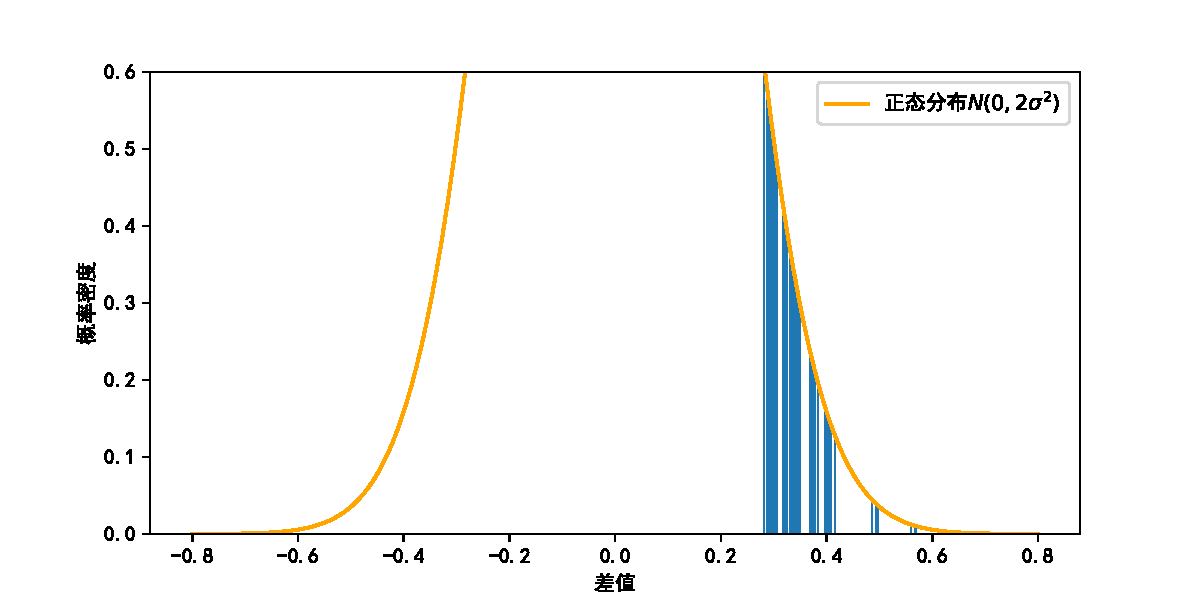
\includegraphics[width=\textwidth]{fig/plottingNormalDistriOfDifference.pdf}
                \caption{差值的分布情况}
                \label{fig:distriOfDifference}
            \end{figure}

            图\ref{fig:distriOfDifference}中的橙色曲线展示了差值的概率分布,35条蓝色竖线表示实际测得最大的35个差值在其中的位置。

            \begin{proposition}
                $$
                \mathcal{D}_{T\left[F_1\right]}(\delta)=\mathcal{D}_{F_2}(\delta)=P_{\sigma_F^2}(\delta),\quad\forall \delta\in\mathbb{R}
                $$
                
                其中“缩放变换” $T$ 满足 $T\left[F_1\right]=F_2$,常数 $\sigma_F$ 约等于 $0.109$ 。

                \label{prop:deltaDistributionOfF2}
            \end{proposition}

        \subsubsection{消除初赛对分数分布的影响}\label{sec:counteringPreliminaryRound}

            这一小节将计算初赛分数线映射为复赛分数后的值,并借助该值计算出:消除初赛的筛选性带来的影响后(即假想初赛并未淘汰一人,所有选手都晋级复赛),复赛的分数分布函数。

            \vspace{1.5ex}

            在\ref{sec:dataOfPreliminaryRound}小节中,已经得到了CSP2019初赛参赛选手的分数数据。由表\ref{tab:noip16to19}中的数据知,在2016到2019四年中,平均每年的初赛晋级人数约为11350;因此我们选择CSP2019初赛全国第11350名的分数,作为假设\ref{ass:preliminaryRoundsOfAllProvincesUnite}中的“全国统一晋级分数线”。

            这里之所以对晋级人数而不是晋级率取平均数,是因为初赛的参赛选手总数受收费、政策等无关因素影响过大,而晋级复赛的人数与复赛获奖的人数呈固定比例,因而相对可靠。

            最终算得分数线为63分。作为参照,CSP2019初赛中,浙江、山东、江苏实际的分数线\footnote{这里给出的是全省分数线,省内各市的分数线可能高于全省分数线}分别为72.5,60,53。

            \vspace{1.5ex}

            下面将这一分数线映射为复赛分数。为了与\ref{sec:parameterOfDeltaDistribution}小节保持一致,这里仍然使用同样的计算方式,并同样采用北京的数据。
            
            我们将计算CSP2019初赛中,北京排名前195名的分数标准差 $\sigma_1$ ,再对(按\ref{sec:parameterOfDeltaDistribution}小节中的方式)映射后的NOIP2018复赛分数计算北京选手前195名的分数标准差 $\sigma_2$ 。然后对于CSP2019初赛分数 $s\in [0,100]$ ,将其映射到 $1-(1-\frac {s}{100})\cdot\sigma_2/\frac{\sigma_1}{100}$ 。这一计算过程基于如下假设:2019年北京选手整体水平,与2018年大体相同。

            对分数线63施加上述变换,得到其对应的复赛分数为$h\approx 0.1035$。另一方面,由命题\ref{prop:deltaDistributionOfF2}可知,任何一名选手的初赛、复赛的(变换后)实际分数之差服从概率分布 $N(0,2\sigma_F^2)$ 。从而,如果假想所有初赛选手都参加了复赛,则对于复赛实际分数为 $t$ 的选手 $p$ ,其初赛分数达到 63 的概率为 $1-R_{2\sigma_F^2}(h-t)$ 。
            
            需要注意,这样得到的概率,是在获得具体的期望值分布前的先验概率。假如已知全体选手的期望分数分布情况,我们可以用贝叶斯公式得到前述选手 $p$ 的期望分数取每一个值的概率,进而得到 $p$ 的初赛分数取每一个值的概率,也就是后验概率。简便起见这里采用先验概率,即使它相比后验概率略失精确。

            记 $F_2^\prime$ 为现实比赛 $B_2$ 在消除初赛的筛选性带来的影响后所对应的理想比赛,则由以上讨论可得:
            $$
            \mathcal{C}_{F_2^\prime}(s)\propto\frac{\mathcal{C}_{F_2}(s)}{1-R_{2\sigma_F^2}(h-s)}=\frac{-\log(s)}{1-R_{2\sigma_F^2}(h-s)},\quad\forall s\in (0,1]
            $$

            上式中之所以使用“正比于”而不是“等于”,是因为分数分布函数表达的是分布“密度”,而不是样本“数量”。计算出对应的比例系数后得到:
            $$
            \mathcal{C}_{F_2^\prime}(s)=\gamma\frac{-\log(s)}{1-R_{2\sigma_F^2}(h-s)},\quad\forall s\in (0,1]
            $$
            其中常数 $\gamma\approx0.549$ ,它使得$\mathcal{C}_{F_2^\prime}$在$[0,1]$上的定积分等于1。

            \begin{figure}[htbp]
                \centering
                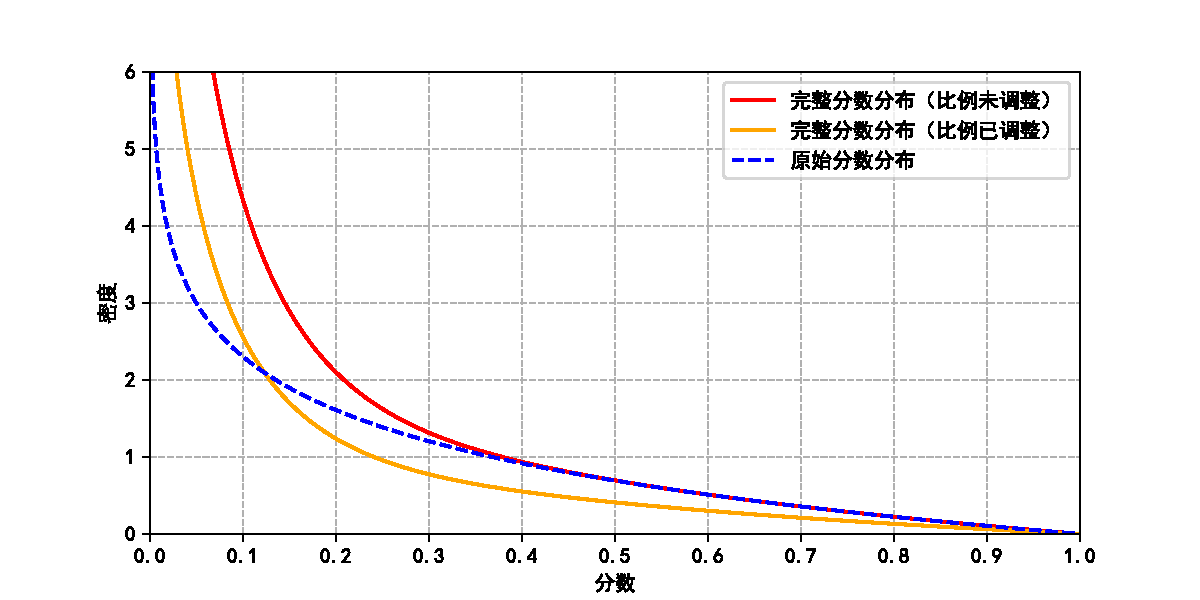
\includegraphics[width=\textwidth]{fig/plottingNewNoipScores.pdf}
                \caption{消除初赛影响前后的分数分布函数}
                \label{fig:curvesBeforeAndAfterCountering}
            \end{figure}

            图\ref{fig:curvesBeforeAndAfterCountering}分别展示了以下三个函数的图像:
            \begin{asparaitem}
                \vspace{1ex}
                \item [\textbf{蓝色}] $f(s)=-\log(s)$,即$\mathcal{C}_{F_2}(s)$或$\mathcal{C}_A(s)$。
                \vspace{1ex}
                \item [\textbf{红色}] $f(s)=\frac{-\log(s)}{1-R_{2\sigma_F^2}(h-s)}$
                \vspace{1ex}
                \item [\textbf{橙色}] $f(s)=\gamma\frac{-\log(s)}{1-R_{2\sigma_F^2}(h-s)}$,即$\mathcal{C}_{F_2^\prime}(s)$。
                \vspace{1ex}
            \end{asparaitem}

            \vspace{1.5ex}

            由\ref{sec:assumptionsOnPreliminaryRound}小节中的讨论知,$\mathcal{C}_A$ 与 $\mathcal{C}_{F_2}$ 相同。同理,如果定义 $A^\prime$ 为:复赛在去除初赛影响后对应的理想比赛(这里采用\textbf{按原本的方式}解读的定义\ref{def:realIdealCorrespondence}),则 $\mathcal{C}_{A^\prime}$ 亦与 $\mathcal{C}_{F_2^\prime}$ 相同。因此有以下命题:

            \begin{proposition}
                $$
                \mathcal{C}_{A^\prime}(s)=\gamma\frac{-\log(s)}{1-R_{2\sigma_F^2}(h-s)},\quad\forall s\in (0,1]
                $$

                其中常数 $\gamma\approx0.549$ ,且 $A^\prime$ 为复赛在去除初赛影响后对应的理想比赛。

                \label{prop:scoreDistributionAfterCountering}
            \end{proposition}

    \subsection{从分数分布还原期望值分布}\label{sec:calculatingXofSecondRound}

        在\ref{sec:counteringPreliminaryRound}小节中得到了 $\mathcal{C}_{A^\prime}(s)$ 的表达式;这一小节将由此计算 $\mathcal{X}_{A^\prime}(x)$ 。

        根据定理\ref{thm:normalityOfOffsetsDistribution},存在 $\sigma>0$ 使得
        $$
        \mathcal{D}_{A^\prime}(\delta)=P_{\sigma^2}(\delta),\quad\forall \delta\in\mathbb{R}
        $$

        进而由命题\ref{prop:scoreDistributionInSimpleContest}得
        \begin{equation}
            \mathcal{C}_{A^\prime}(s)=\int\limits_0^1 \mathcal{X}_{A^\prime}(x)P_{\sigma^2}(s-x)\mathrm{d}x,\quad\forall s\in\mathbb{R}
            \label{formula:fromXtoC_beforeUpd}
        \end{equation}

        于是,我们可以根据\eqref{formula:fromXtoC_beforeUpd},由 $\mathcal{C}_{A^\prime}$ 逆推出 $\mathcal{X}_{A^\prime}$ 。

        但是在这个问题中,期望分数接近0的选手占了总数中相当的比重,因此若单纯按\eqref{formula:fromXtoC_beforeUpd}计算,则“负分数”问题(在\ref{sec:keyAssumptions}小节末尾有所提及)会变得十分显著。为解决这一问题,我们对于每一名选手,将其分数的概率分布中负的一段截掉,再将剩余部分的概率密度函数乘以某个系数,以使得乘完后剩余部分的总概率为1。若一名选手期望分数为 $x$ ,则容易证明:对该名选手而言,在上述过程中使用的系数$c(x)$等于 $$\left(\int\limits_0^1 P_{\sigma^2}(t-x)\mathrm{d}t\right)^{-1}=\left(R_{\sigma^2}(1-x)-R_{\sigma^2}(0-x)\right)^{-1}$$

        于是$\mathcal{C}_{A^\prime}$与$\mathcal{X}_{A^\prime}$间的关系被更新为
        \begin{equation}
            \mathcal{C}_{A^\prime}(s)=\int\limits_0^1 \mathcal{X}_{A^\prime}(x)\cdot\frac{P_{\sigma^2}(s-x)}{R_{\sigma^2}(1-x)-R_{\sigma^2}(0-x)}\mathrm{d}x,\quad\forall s\in\mathbb{R}
            \label{formula:fromXtoC}
        \end{equation}

        \vspace{1.5ex}

        在进行逆推之前,先测量 $\sigma$ 的值。我们获取了CSP2019复赛全体选手的民间分数(零分选手被去除,共计12108人获得非零分数),并按以下步骤进行测量:
        \begin{asparaenum}[\bfseries{步骤} 1.]
            \item 将每名选手每一天的分数除以当天最高分(两天最高分均为满分300分),再将每一天的所有分数做变换,以使得两天的分数分布分别呈对数曲线状。具体变换方式与\ref{sec:parameterOfDeltaDistribution}小节中相同;经过变换后,两天分别对应的理想比赛应当与 $A^\prime$ 相同。
            \item 对每名选手计算两天分数之差,计算所有这些差值的标准差 $\sigma_0$ 。
        \end{asparaenum}

        \vspace{1.5ex}

        与\ref{sec:parameterOfDeltaDistribution}小节中类似,同一名选手的单日分数(变换后的分数),应该服从标准差为 $\sigma_1=\frac {\sigma_0}{\sqrt 2}$ 的正态分布。记CSP2019复赛第一天、第二天,这两个现实比赛分别为 $D_1,D_2$ ,则 $\Delta_{D_1},\Delta_{D_2}$ 服从正态分布 $N(0,\sigma_1^2)=N(0,\frac {\sigma_0^2}{2})$ 。记现实比赛 $D$ 为CSP2019复赛(两天综合),则有 $\Delta_D=\frac{\Delta_{D_1}+\Delta_{D_2}}2$ 。进而由引理\ref{lem:stddevOfSumOfIndependentVars}:
        
        \begin{align*}
            \mathrm{Stddev}\left[\Delta_D\right]&=\frac{\sqrt{\mathrm{Stddev}\left[\Delta_{D_1}\right]^2+\mathrm{Stddev}\left[\Delta_{D_2}\right]^2}}2 \\
                                                &=\frac{\sqrt{2}\sigma_1}{2} \\
                                                &=\frac{\sigma_0}{2}
        \end{align*}
        
        得到 $\sigma=\frac {\sigma_0}2$ 。换句话说:同一名选手在CSP2019复赛中(变换后)的分数波动,服从标准差为 $\sigma=\frac {\sigma_0}2$ 的正态分布。
        
        最终算得 $\sigma\approx0.078$ 。

        \vspace{1.5ex}

        从 $\mathcal{C}_{A^\prime}$ 和 $\mathcal{D}_{A^\prime}$ 逆推出 $\mathcal{X}_{A^\prime}$ 难以精确地实现,因此这里只能近似地计算 $\mathcal{X}_{A^\prime}$ 在许多个离散的点处的点值。

        我们将区间 $(0,1]$ 作500等分,并设立500个未知数 $x_{1\cdots 500}$ ,分别表示在500个分点处 $\mathcal{X}_{A^\prime}$ 的取值。另一方面,我们在\eqref{formula:fromXtoC}中将$s$取遍每一个分点,由此得到500个等式限制;注意到仅凭 $x_{1\cdots 500}$ 无法表示出\eqref{formula:fromXtoC}中的定积分,因此定积分被换成离散的求和。在作了这样的“离散化”之后,原先的等式显然不再成立,因此改为最小化所有每一个等式两端之差的平方和。为了避免无意义的结果,我们额外加入了关于序列 $x_{1\cdots 500}$ 非负性和“光滑性”的限制;后者通过序列 $x_{1\cdots 500}$ 的高阶差分来表示。

        上述问题最终归结到了一个二次规划模型的求解;可以证明其为凸二次规划,因此任何一个极值点都是最值点。最优化方法采用SciPy提供的信赖域算法的实现\cite{scipy_minimize}。用于计算的程序和最终算得的点值 $x_{1\cdots 500}$ ,可以在本文开头的链接中找到。

        观察所得的500个点值,发现:
        \begin{asparaenum}
            \item 在与0紧邻的位置处,点值明显大于其他位置。
            \item 在其余位置处,点值构成一条平滑的曲线。计算发现这些点值近似地符合二次函数 $f(x)=ax^2+bx+c$ ,其中 $a\approx 1.697,b\approx -3.352,c\approx 1.655$ 。图\ref{fig:quadFuncOfXAprime}展示了该函数的图像。
        \end{asparaenum}

        \begin{figure}[htbp]
            \centering
            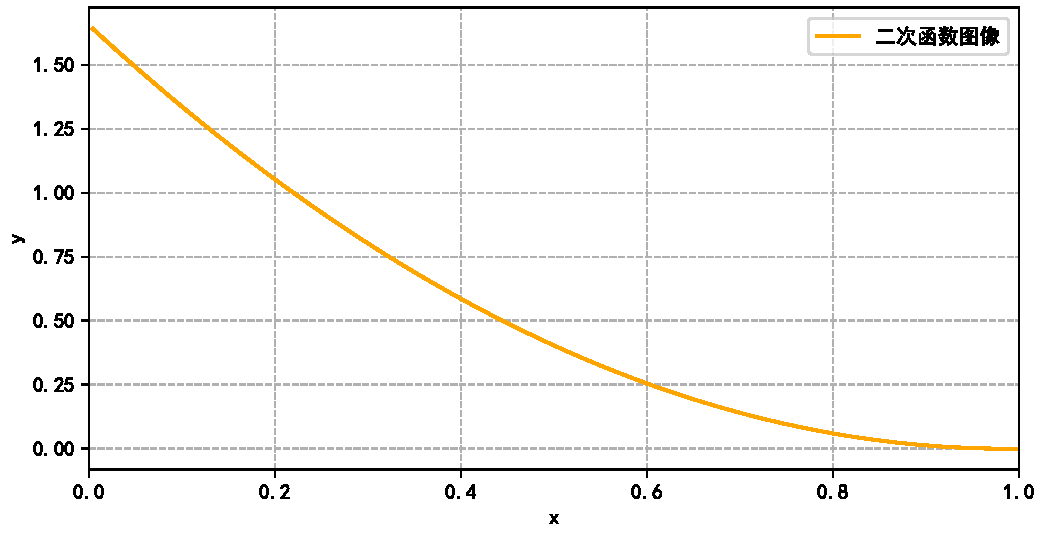
\includegraphics[width=\textwidth]{fig/plottingQuadFuncOfXAprime.pdf}
            \caption{二次函数$f(x)=ax^2+bx+c$}
            \label{fig:quadFuncOfXAprime}
        \end{figure}

        至此,我们得到了函数$\mathcal{X}_{A^\prime}$的表达式。

        \begin{theorem}
            对于 $x\in(\epsilon,1]$ 有 $\mathcal{X}_{A^\prime}(x)=ax^2+bx+c$ ,其中 $a\approx 1.697,b\approx -3.352,c\approx 1.655$ ,$\epsilon$ 为某个小常数,$A^\prime$ 为复赛在去除初赛影响后对应的理想比赛。

            \label{thm:formulaforXAprime}
        \end{theorem}

        最后,如本节开头所说,本节的目标旨在估计而非精准计算,所得的结果仅能反映趋势而不保证精确;这对上述定理也同样成立。

\section{关于比赛名次的讨论}

    本节中研究关于比赛名次的性质,这些性质可以为选手的比赛策略制订和日常训练导向提供参考。

    \subsection{比赛名次与实际水平的关系}\label{sec:relationBetweenCapabilityAndRanking}

        一名选手在比赛得分上的波动,导致了他在比赛名次上的波动。考虑到各种奖项的颁发都是以名次而非得分为主要依据,研究选手比赛名次的概率分布就显得格外重要。
        
        具体地说,对于 $A,B$ 为一对互相对应的理想比赛和现实比赛,在这一小节中我们考虑:在该场比赛中额外加入一名选手 $p$ (该选手得分的概率分布给定),则他的名次的概率分布为何。特别地,我们研究两个自变量(选手$p$的\emph{期望分数}和\emph{分数波动幅度})对两个因变量(选手$p$的\emph{期望名次}和\emph{中位名次})的影响。

        本节中考虑的 $B$ 均为COI/IOI赛制的信息学比赛。于是由定理\ref{thm:normalityOfOffsetsDistribution}, $\Delta_B$ 和选手 $p$ 的得分都服从正态分布。

        \subsubsection{期望分数与比赛名次的关系}

            记随机变量 $C_p$ 为 $p$ 的(与 $B$ 中的选手分数一起,按定义\ref{def:realIdealCorrespondence}中的方式变换过后的)分数,设其服从期望值为 $\mu$ 、标准差为 $\sigma$ 的正态分布,并用 $\mathcal{D}_p$ 来表示 $C_p-\mu$ 的概率密度函数。

            令随机变量 $U_p$ 表示: $B$ 中有多大比例的选手实际得分高于 $p$ 的实际得分(例如 $U_p=0.5$ 表示 $B$ 中恰一半的选手实际得分高于 $p$)。

            令实数 $V_p$ 表示: $B$ 中有多大比例的选手期望得分高于 $p$ 的期望得分(例如 $V_p=0.5$ 表示 $B$ 中恰一半的选手期望得分高于 $p$)。

            此外设 $\Delta_B$ 服从正态分布 $N(0,\sigma_B^2)$ ,从而对任意 $\delta$ 有 $\mathcal{D}_A(\delta)=P_{\sigma_B^2}(\delta)$ 。

            \vspace{1.5ex}

            这一小节中将对变化的 $\mu$ ,考察以下两个量的变化趋势:
            \begin{asparaitem}
                \item $D_1=\mathrm{E}\left[U_p\right]-V_p$
                \item $D_2=\mathrm{Med}\left[U_p\right]-V_p$,其中\textbf{中位名次} $\mathrm{Med}\left[U_p\right]$ 满足 $\mathrm{Pr}\left[U_p>\mathrm{Med}\left[U_p\right]\right]=0.5$ 
            \end{asparaitem}

            \vspace{1.5ex}

            对于$\mathrm{E}\left[U_p\right]$不难发现:
            \begin{align*}
                \mathrm{E}\left[U_p\right]
                &=\int\limits_0^1 \mathcal{X}_A(x)\left(\iint\limits_{\left\{(\delta_1,\delta_2):\mu+\delta_1\leq x+\delta_2\right\}} \mathcal{D}_p(\delta_1)\mathcal{D}_A(\delta_2)\mathrm{d}(\delta_1,\delta_2)\right)\mathrm{d}x \\
                &=\int\limits_0^1 \mathcal{X}_A(x)\left(\iint\limits_{\left\{(\delta_1,\delta_2^-):\delta_1+\delta_2^-\leq x-\mu\right\}} P_{\sigma^2}(\delta_1)P_{\sigma_B^2}(-\delta_2^-)\mathrm{d}(\delta_1,\delta_2^-)\right)\mathrm{d}x \\
                &=\int\limits_0^1 \mathcal{X}_A(x)\left(\int\limits_{-\infty}^{x-\mu} P_{\sigma^2+\sigma_B^2}(\delta)\mathrm{d}\delta\right)\mathrm{d}x \\
                &=\int\limits_0^1 \mathcal{X}_A(x)R_{\sigma^2+\sigma_B^2}(x-\mu) \mathrm{d}x
            \end{align*}

            而对于$\mathrm{Med}\left[U_p\right]$有
            \begin{align}
                \mathrm{Med}\left[U_p\right]
                &=\int\limits_{\mu}^{+\infty} \mathcal{C}_A(s)\mathrm{d}s \label{formula:whatMedIs}\\
                &=\int\limits_0^1 \mathcal{X}_A(x)R_{\sigma_B^2}(x-\mu) \mathrm{d}x \notag
            \end{align}

            其中等式\eqref{formula:whatMedIs}成立的理由是
            \begin{align*}
            &\phantom{=\ }\mathrm{Pr}\left[U_p>\int\limits_{\mu}^{+\infty} \mathcal{C}_A(s)\mathrm{d}s\right] \\
            &=\mathrm{Pr}\left[C_p>\mu\right] \\
            &=0.5
            \end{align*}

            由此可以对给定的 $\mu,\sigma,\mathcal{X}_A$ 计算 $D_1,D_2$ 的值。

            \vspace{1.5ex}

            \begin{figure}[htbp]
                \centering
                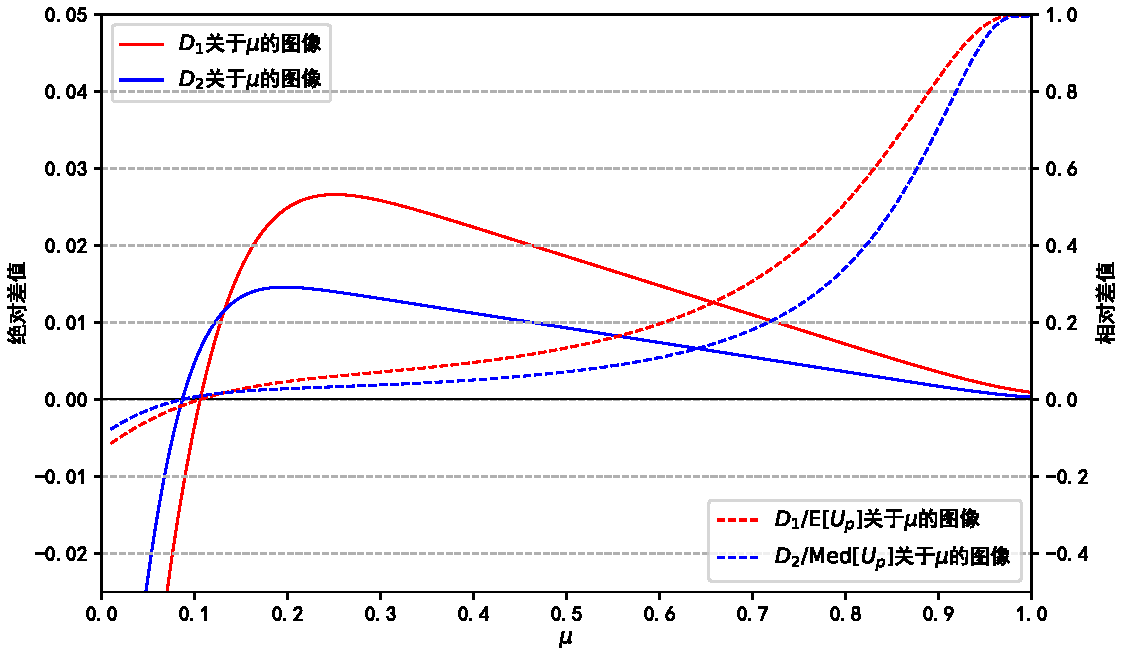
\includegraphics[width=\textwidth]{fig/plottingD_1D_2.pdf}
                \caption{$D_1,D_2$的图像,当$A$为定理\ref{thm:formulaforXAprime}中的$A'$时}
                \label{fig:plottingD_1D_2forAprime}
            \end{figure}

            \begin{figure}[htbp]
                \centering
                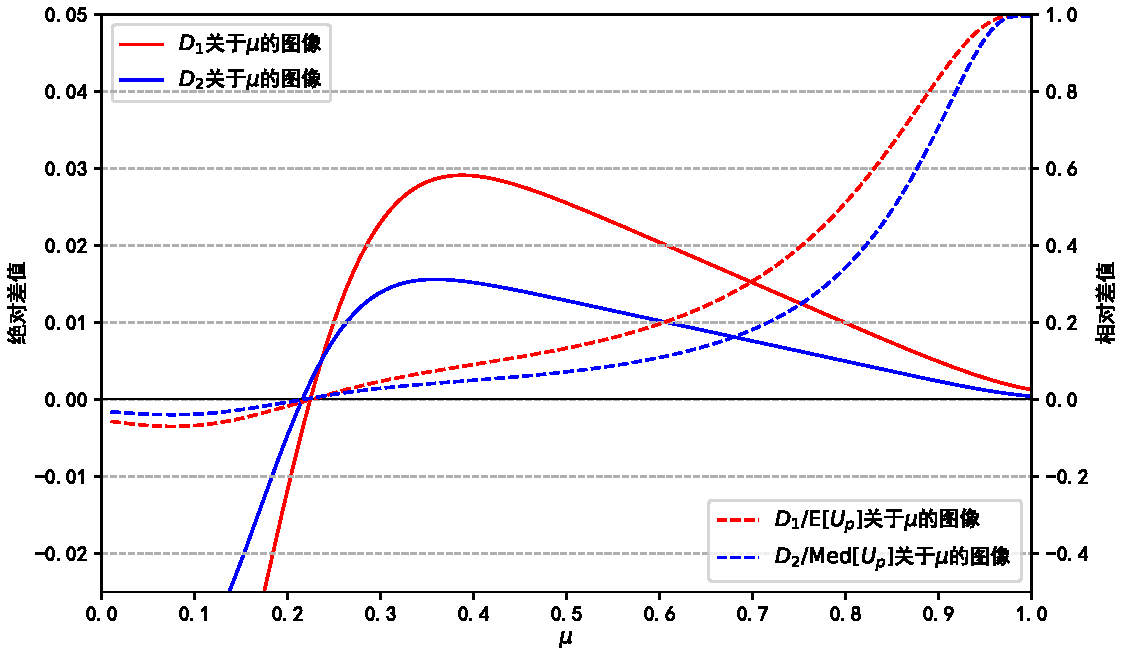
\includegraphics[width=\textwidth]{fig/plottingNoipD_1D_2.pdf}
                \caption{$D_1,D_2$的图像,当$A$对应联赛复赛时}
                \label{fig:plottingD_1D_2forNoip}
            \end{figure}

            \begin{figure}[htbp]
                \centering
                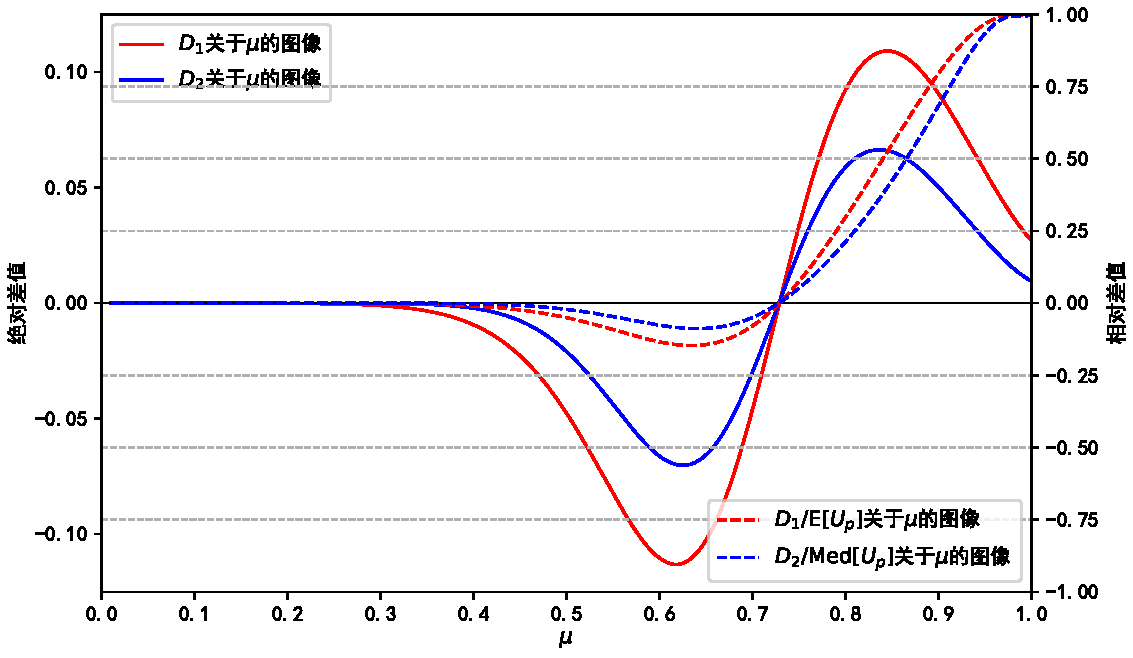
\includegraphics[width=\textwidth]{fig/plottingNoiD_1D_2.pdf}
                \caption{$D_1,D_2$的图像,当$A$对应NOI时}
                \label{fig:plottingD_1D_2forNoi}
            \end{figure}

            取理想比赛 $A$ 为定理\ref{thm:formulaforXAprime}中“复赛在去除初赛影响后对应的理想比赛”$A'$、取$\sigma=\sigma_B\approx 0.078$(该数值来自于\ref{sec:calculatingXofSecondRound}小节中的测量),则 $D_1,D_2$ 关于 $\mu$ 的图像如图\ref{fig:plottingD_1D_2forAprime}。这里对于期望分数小于(定理\ref{thm:formulaforXAprime}中的)$\epsilon$的选手,将他们从$\mathcal{X}_A$中剔除,并将 $\mathcal{X}_A$ 剩余部分的点值乘上某个系数,以使得其在$[0,1]$上定积分仍为$1$。这样得到的$\mathcal{X}_A$为二次函数。此外,$D_1,D_2$ 本身是“绝对差值”,图中还用虚线绘制了“相对差值”$\frac{D_1}{\mathrm{E}\left[U_p\right]},\frac{D_2}{\mathrm{Med}\left[U_p\right]}$的图像。

            \vspace{1.5ex}

            图\ref{fig:plottingD_1D_2forAprime}所考虑的情况是:现实比赛$B$的参赛人群为期望分数达到$\epsilon$的\textbf{全体}信息学选手。但是对于实际中的比赛,其参赛选手往往是经过选拔的;以下将研究此类比赛。

            简便起见,我们作如下假设:现实比赛$B$的参赛人群,是期望分数达到$\epsilon$的\textbf{全体}信息学选手,经过一场现实比赛 $C$ 的选拔后达到分数线的那些;其中 $C$ 所对应的理想比赛与(定理\ref{thm:formulaforXAprime}中的) $A'$ 完全相同,且分数线为 $\textit{thres}\in[0,1]$ 。

            由此易知,对于一名期望分数为 $\mu_q\in [0,1]$ 的选手 $q$ ,他达到分数线的概率为 $1-R_{(0.078)^2}(\textit{thres}-\mu_q)$ 。进而得到:
            $$
            \mathcal{X}_A(x)\propto (ax^2+bx+c)\left(1-R_{(0.078)^2}(\textit{thres}-x)\right),\quad\forall x\in [0,1]
            $$

            其中 $a,b,c$ 为定理\ref{thm:formulaforXAprime}中的系数。

            \vspace{1.5ex}

            为模拟联赛复赛的情况,取 $\textit{thres}=0.1053$ (该数值为\ref{sec:counteringPreliminaryRound}小节中的计算结果),此时 $D_1,D_2$ 的图像如图\ref{fig:plottingD_1D_2forNoip};为模拟NOI的情况,取 $\textit{thres}=0.7$ (计算发现近几年联赛中得分高于该数值的选手人数与NOI的参赛人数相近,故选择该数值),此时 $D_1,D_2$ 的图像如图\ref{fig:plottingD_1D_2forNoi}。

            \vspace{1.5ex}

            观察图\ref{fig:plottingD_1D_2forAprime}、图\ref{fig:plottingD_1D_2forNoip}和图\ref{fig:plottingD_1D_2forNoi},可以得到以下结论:

            \begin{tcolorbox}[colback=white,colframe=black,boxrule=0.5pt,arc=0pt]
                在一场信息学比赛中,对任何一名期望得分“不太低”的选手,他的期望名次、中位名次,均\textbf{差于}他的实际水平(以期望得分来衡量)在全体参赛选手中的位次。这一现象随着该名选手期望得分的升高而越发明显,在高分段尤其显著。
            \end{tcolorbox}

            这一点也很容易直观理解:由于分数分布大体上呈现“低分稠密、高分稀疏”的状态,所以期望得分接近但低于 $p$ 的选手数量,会超过期望得分接近且高于 $p$ 的选手数量。进而,\emph{将} $p$ 反超的人数,就会大于\emph{被} $p$ 反超的人数。

        \subsubsection{分数波动幅度与比赛名次的关系}

            这一小节中将考察 $\sigma$ 的变化对 $\mathrm{E}\left[U_p\right]$ 的影响。注意到 $\sigma$ 的变化不影响 $\mathrm{Med}\left[U_p\right]$ 的值,所以这里不考虑 $\mathrm{Med}\left[U_p\right]$ 。

            记 $\mathrm{E}\left[U_p\right](\mu_0,\sigma_0)$ 为 $\mu=\mu_0,\sigma=\sigma_0$ 时 $\mathrm{E}\left[U_p\right]$ 的取值,则我们将考察以下函数:
            $$
            F(\mu_0,\sigma_0)=\frac{\mathrm{E}\left[U_p\right](\mu_0,\sigma_0)-\mathrm{E}\left[U_p\right](\mu_0,0)}{\mathrm{E}\left[U_p\right](\mu_0,\sigma_0)+\mathrm{E}\left[U_p\right](\mu_0,0)}
            $$

            函数$F$的含义是$\mathrm{E}\left[U_p\right]$随$\sigma$的变化而产生的增量;这里的增量用$\mathrm{E}\left[U_p\right](\mu_0,\sigma_0)$与$\mathrm{E}\left[U_p\right](\mu_0,0)$的相对差值来描述,由于二者中任何一者都可能远小于对方,故分母上取二者之和而非二者之一。

            \vspace{1.5ex}

            上一小节中对三个比赛分别绘制了 $D_1,D_2$ 的图像;这里我们对同样的三个比赛绘制 $F$ 的图像,见图\ref{fig:plottingD_1D_2forAprimeWrtSigma}、图\ref{fig:plottingD_1D_2forNoipWrtSigma}和图\ref{fig:plottingD_1D_2forNoiWrtSigma}。图中底部的线条为上方曲面的等高线。此外请注意图中坐标轴的方向。

            \begin{figure}[p]
                \centering
                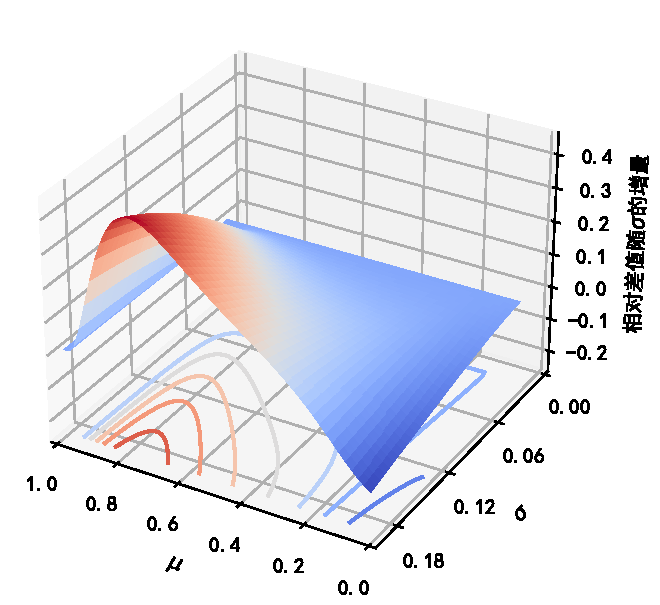
\includegraphics[width=\textwidth]{fig/plottingD_1D_2WrtSigma.pdf}
                \caption{$F$的图像,当$A$为定理\ref{thm:formulaforXAprime}中的$A'$时}
                \label{fig:plottingD_1D_2forAprimeWrtSigma}
            \end{figure}

            \begin{figure}[p]
                \centering
                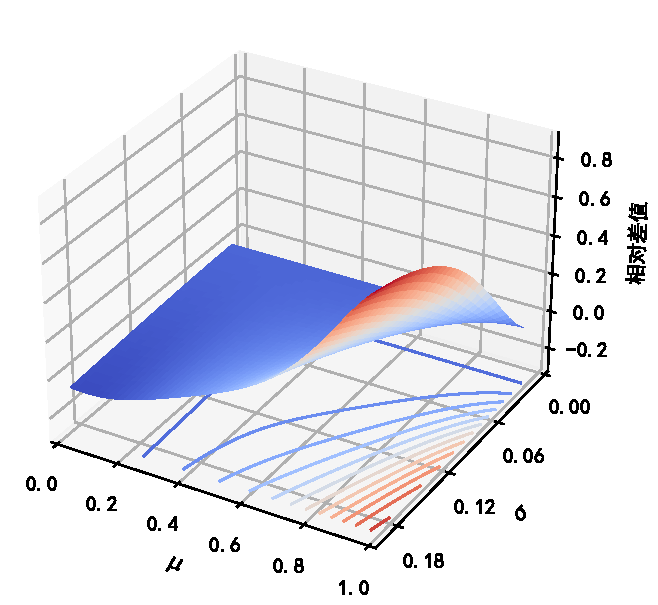
\includegraphics[width=\textwidth]{fig/plottingNoipD_1D_2WrtSigma.pdf}
                \caption{$F$的图像,当$A$对应联赛复赛时}
                \label{fig:plottingD_1D_2forNoipWrtSigma}
            \end{figure}

            \begin{figure}[p]
                \centering
                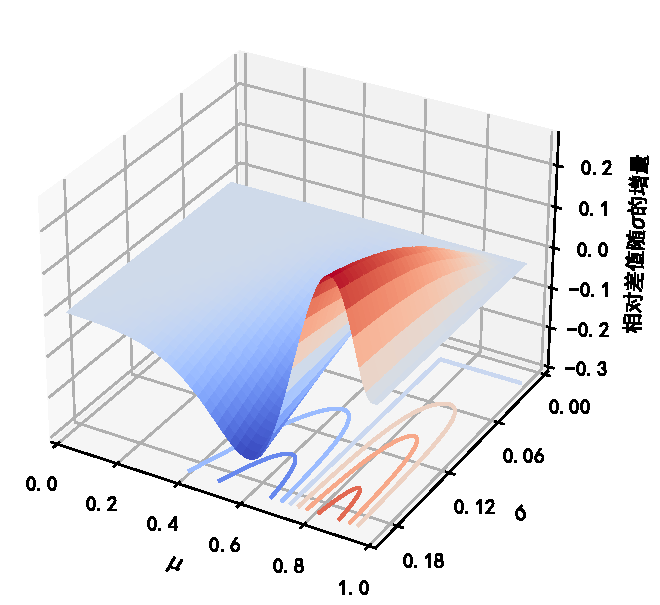
\includegraphics[width=\textwidth]{fig/plottingNoiD_1D_2WrtSigma.pdf}
                \caption{$F$的图像,当$A$对应NOI时}
                \label{fig:plottingD_1D_2forNoiWrtSigma}
            \end{figure}

            观察三个图像,可以得到以下结论:

            \begin{tcolorbox}[colback=white,colframe=black,boxrule=0.5pt,arc=0pt]
                在一场信息学比赛中,对任何一名期望得分“不太低”的选手,若他的期望得分固定,则当他的分数分布的标准差提高时,他的期望名次变差。这一现象随着该名选手期望得分的升高而越发明显,在高分段尤其显著。
            \end{tcolorbox}

    \subsection{多日比赛总名次与单日名次的关系}\label{sec:relationBetweenEachDayAndTotal}

        大多数信息学比赛都包括两天或更多的比赛日,而对于其中的大部分比赛,选手在每日考试后也都能直接或间接地知道自己当日的大致排名。这种情况下,一名选手在先前的考试日中的排名,对他在之后的考试日中的策略制定是一个重要信息。但要想有效利用这一信息,首先需要了解多日比赛总名次与单日名次之间的关系,而这正是本小节的目标。

        \vspace{1.5ex}

        先给出这一小节用到的模型:现实比赛 $B_{1\cdots k}$ 分别表示每一天的比赛,它们对应同一个理想比赛 $A$ 。一名选手的\textbf{总分}定义为:他在 $B_{1\cdots k}$ 中的分数 $\textit{score}_{1\cdots k}$ (满足 $\textit{score}_i\in[0,1]$ )的加权平均数 $w_1\textit{score}_1+\cdots+w_k\textit{score}_k$ (满足 $w_1+\cdots+w_k=1$ )。

        在实际中,每天的比赛在难度、区分度上可能有差异,因此仅可以认为各天的比赛(所对应的理想比赛)\emph{缩放等价}而不是完全相同;但通过引入权值 $w_{1\cdots k}$ ,可以将这些比赛“标准化”。也就是说, $w_{1\cdots k}$ 在此处相当于“缩放系数”,与等价映射中的一次项系数作用相同。

        设 $\Delta_{B_i}$ 服从正态分布 $N(0,\sigma_B^2)$ 。以下我们关注比赛中的一名特定选手 $p$ ,记他各天的分数为 $\textit{score}_{1\cdots k}$ 、各天的名次为 $\textit{rank}_{1\cdots k}$ (满足 $\textit{rank}_i\in [0,1]$ ,定义方式与上一节中的 $U_p$ 相同),我们将尝试从 $\textit{rank}_{1\cdots k}$ 近似地计算 $p$ 的\emph{总分}名次 $\textit{rank}_{\textit{total}}\in [0,1]$ 。
        
        这里我们还要求:
        \begin{asparaitem}
            \item $\mathcal{X}_A(x)=\left(a^\prime x^2+b^\prime x+c^\prime\right)\left(1-R_{\sigma_P^2}(\textit{thres}-x)\right)$ ,其中 $(a^\prime,b^\prime,c^\prime)\propto (a,b,c)$ 为常系数、$\textit{thres},\sigma_P$ 为某两个不关心其具体取值的常数。
            \item 注意到对足够大的 $x$ (不妨划定为 $x\geq T$ ,其中 $T$ 为某个不关心其具体取值的常数)有 $\mathcal{X}_A(x)\approx a^\prime x^2+b^\prime x+c^\prime$ 。我们要求 $p$ 的得分和名次足够高,以致于 $\mathcal{X}_A(x)$ 在 $x<T$ 的部分对答案几乎没有影响。
        \end{asparaitem}

        \subsubsection{$\sigma_B=0$的情况}

            在这一小节中,假设 $\sigma_B=0$ 。严格地说, $\sigma_B$ 必须是正数,否则 $N(0,\sigma^2)$ 就并非良定义;但这里 $\sigma_B=0$ 仅用来表达 $\mathcal{C}_A=\mathcal{X}_A$ ,故暂且忽略这一问题。

            通过对系数 $a^\prime,b^\prime,c^\prime$ 的计算,发现 $a^\prime x^2+b^\prime x+c^\prime\approx a^\prime(x-1)^2$ ,于是可以得到:
            \begin{align*}
                \textit{rank}_i
                &=\int\limits_{\textit{score}_i}^1 \mathcal{C}_A(s) \mathrm{d}s \\
                &\approx\int\limits_0^{1-\textit{score}_i} a^\prime s^2 \mathrm{d}s \\
                &=\frac{a^\prime\left(1-\textit{score}_i\right)^3}3
            \end{align*}

            所以有
            $$
            1-\textit{score}_i\approx\sqrt[3]{\frac{3\textit{rank}_i}{a^\prime}}
            $$

            进而 $p$ 的总分 $\textit{score}_{\textit{total}}$ 满足
            $$
            1-\textit{score}_{\textit{total}}\approx\sum\limits_{i=1}^k w_i\sqrt[3]{\frac{3\textit{rank}_i}{a^\prime}}
            $$

            最后
            \begin{align*}
                \textit{rank}_{\textit{total}}
                &\approx\frac{a^\prime(1-\textit{score}_{\textit{total}})^3}3 \\
                &\approx\frac{a^\prime}{3}\cdot\left(\sum\limits_{i=1}^k w_i\sqrt[3]{\frac{3\textit{rank}_i}{a^\prime}}\right)^3 \\
                &=\left(\sum\limits_{i=1}^k w_i\sqrt[3]{\textit{rank}_i}\right)^3
            \end{align*}

            注意到上式的左右两边是齐次的,所以,若将所有$\textit{rank}_{1\cdots k}$和$\textit{rank}_{\textit{total}}$同时乘以常数,则正确性不会受影响。因此即使取$\textit{rank}_{1\cdots k}$和$\textit{rank}_{\textit{total}}$为“原始排名”(即分数高于 $p$ 的人数),上式仍然成立。
            
            \vspace{1.5ex}

            得到结论:

            \begin{tcolorbox}[colback=white,colframe=black,boxrule=0.5pt,arc=0pt]
                若忽略参赛选手分数的波动(也就是假设,除 $p$ 以外的任何选手在任何一天中都恰会考出自己的期望得分),则对于得分足够高的选手 $p$ ,其总名次约等于每日名次的\emph{$1/3$次加权幂平均}。
            \end{tcolorbox}

            结合幂平均不等式\cite{wiki_powerMean},可以得到如下推论:
            
            \begin{tcolorbox}[colback=white,colframe=black,boxrule=0.5pt,arc=0pt]
                在上一结论的条件下,选手 $p$ 的总名次一定不差于(即数值上不大于)每日名次的加权平均数,取等仅当每日名次相同。更进一步,在名次加权平均数固定的情况下,名次波动幅度越大,总名次一般越好(即数值上越小);换句话说,对单场比赛而言,前进$n$名对总名次的正面影响,一般大于后退$n$名对总名次的负面影响。
            \end{tcolorbox}

        \subsubsection{$\sigma_B>0$的情况}

            这一小节中考虑 $\sigma_B>0$ 的情况。

            \vspace{1.5ex}
            
            首先,为了能够直接确定系数 $a^\prime,b^\prime,c^\prime$ ,我们不妨取 $\textit{thres}$ 为 $-\infty$ ,也就是说对任何 $x\in [0,1]$ 有 $\mathcal{X}_A(x)=a^\prime x^2+b^\prime x+c^\prime$ 。注意到对于$\mathcal{X}_A(x)$在$x\in [T,1]$的部分而言,$\textit{thres}$ 的变化只相当于对这一部分函数值作等比例缩放;而稍后会看到,对 $\mathcal{X}$ 和 $\mathcal{C}$ 的函数值的等比例缩放,不会影响后续推导的正确性。因此,钦定 $\textit{thres}$ 的取值不会影响一般性。

            \vspace{1.5ex}

            为了使得后续推导成为可能,需要先对函数$\mathcal{C}_A$作近似,以简化其形式。

            对于确定的 $\sigma_B$ ,可以计算得到实数 $r(\sigma_B)\geq 1$ 和 $a(\sigma_B)\geq 0$ ,以使得函数 $f_{\sigma_B}(s)=a(\sigma_B)(r(\sigma_B)-s)^2$ 的图像与 $\mathcal{C}_A$ 尽可能贴近(即残差平方和最小)。实验发现:
            $$
            \max\limits_{\sigma_B\in (0,0.4],s\in [0.6,1]} \left|f_{\sigma_B}(s)-\mathcal{C}_A(s)\right|\approx 0.02
            $$

            由此可见,这一近似的效果十分优秀。回忆到我们只关注“足够高”的那一部分分数分布,因此在上式中只考虑 $s\geq 0.6$ 。

            \begin{figure}[htbp]
                \centering
                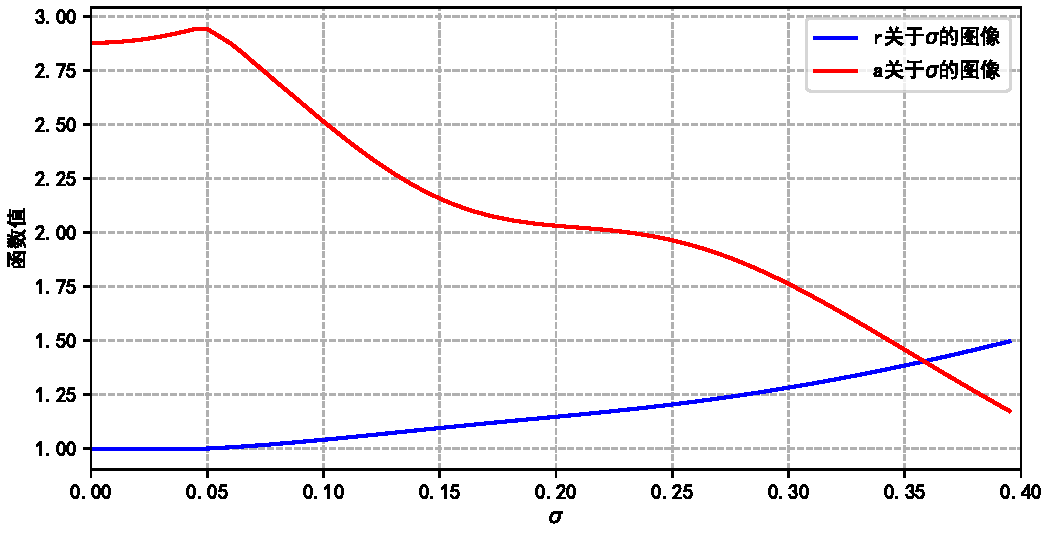
\includegraphics[width=\textwidth]{fig/plottingAandR.pdf}
                \caption{函数$a(\sigma)$和$r(\sigma)$的图像}
                \label{fig:plottingAandR}
            \end{figure}

            图\ref{fig:plottingAandR}展示了函数$a(\sigma)$和$r(\sigma)$的图像。可以看到,前者大体上递降,而后者则递增。

            \vspace{1.5ex}

            将全部 $k$ 个比赛合并视为一个现实比赛 $B_{\textit{total}}$ ,以下计算(服从正态分布的)随机变量 $\Delta_{B_{\textit{total}}}$ 的标准差 $\sigma_{\textit{total}}$ 。
            \begin{align*}
                \sigma_{\textit{total}}
                &=\mathrm{Stddev}\left[\sum\limits_{i=1}^k w_i\Delta_{B_i}\right] \\
                &=\sqrt{\sum\limits_{i=1}^k \mathrm{Stddev}\left[w_i\Delta_{B_i}\right]^2} \\
                &=\sqrt{\sum\limits_{i=1}^k w_i^2\sigma_B^2} \\
                &=\sqrt{\sum\limits_{i=1}^k w_i^2}\cdot\sigma_B
            \end{align*}

            特别地,当权重 $w_i$ 全部相等时,$\sigma_{\textit{total}}=k^{-1/2}\sigma_B$ 。

            \vspace{1.5ex}

            接下来类比上一小节进行推导。注意到$\mathcal{C}_A(s)$在$s\in (1,r]$的部分也要纳入考虑。

            \begin{align*}
                \textit{rank}_i
                &=\int\limits_{\textit{score}_i}^r(\sigma_B) \mathcal{C}_A(s) \mathrm{d}s \\
                &\approx\int\limits_0^{r(\sigma_B)-\textit{score}_i} a(\sigma_B) s^2 \mathrm{d}s \\
                &=\frac{a(\sigma_B)\left(r(\sigma_B)-\textit{score}_i\right)^3}3
            \end{align*}
            \begin{align*}
                r(\sigma_B)-\textit{score}_{\textit{total}}
                &=\sum\limits_{i=1}^k w_i\left(r(\sigma_B)-\textit{score}_i\right) \\
                &\approx\sum\limits_{i=1}^k w_i\sqrt[3]{\frac{3\textit{rank}_i}{a(\sigma_B)}}
            \end{align*}
            \begin{align*}
                \textit{rank}_{\textit{total}}
                &\approx\frac{a(\sigma_{\textit{total}})(r(\sigma_{\textit{total}})-\textit{score}_{\textit{total}})^3}3 \\
                &\approx\frac{a(\sigma_{\textit{total}})}{3}\cdot\left(r(\sigma_{\textit{total}})-r(\sigma_B)+\sum\limits_{i=1}^k w_i\sqrt[3]{\frac{3\textit{rank}_i}{a(\sigma_B)}}\right)^3 \\
                &=\frac{a(\sigma_{\textit{total}})\left(r(\sigma_{\textit{total}})-r(\sigma_B)\right)}{3}+\frac{a(\sigma_{\textit{total}})}{a(\sigma_B)}\left(\sum\limits_{i=1}^k w_i\sqrt[3]{\textit{rank}_i}\right)^3
            \end{align*}

            发现总名次$\textit{rank}_{\textit{total}}$是关于$\big(\sum_{i=1}^k w_i\sqrt[3]{\textit{rank}_i}\big)^3$ 的一次函数。接着注意到$\sigma_{\textit{total}}<\sigma_B$,故由$a(\sigma),r(\sigma)$的增减性可知,该一次函数的一次项系数大于等于1,而常数项小于等于0;因此自变量和因变量的大小关系无法直接确定。

            \begin{figure}[htbp]
                \centering
                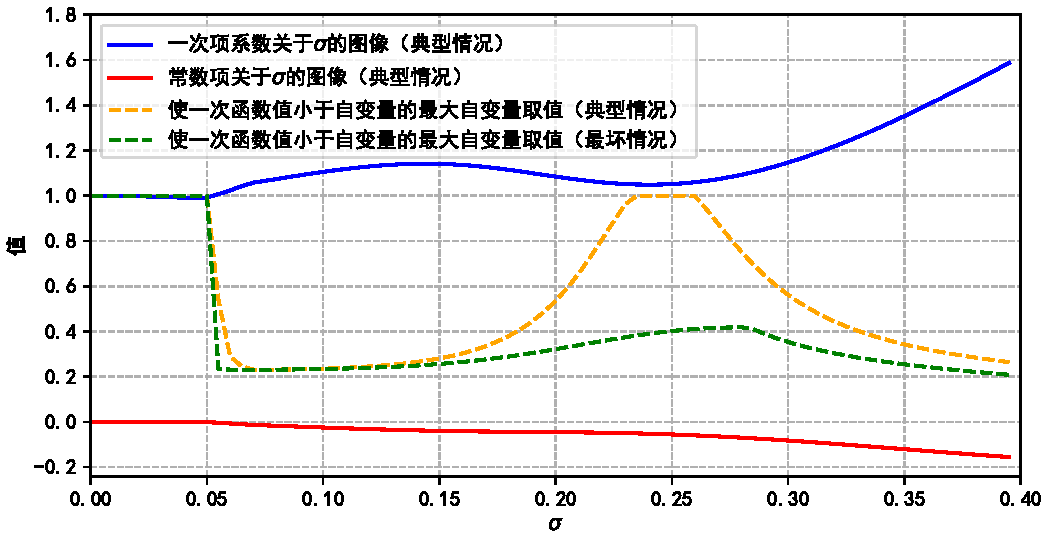
\includegraphics[width=\textwidth]{fig/plottingKandB.pdf}
                \caption{一次函数的系数,以及大小关系改变的阈值}
                \label{fig:plottingKandB}
            \end{figure}

            图\ref{fig:plottingKandB}展示了以下4个量关于$\sigma_B$的图像:
            \begin{asparaitem}
                \vspace{1ex}
                \item [\textbf{蓝色}] 在\emph{典型情况}下(指的是$k=2,w_1=w_2$时的情况,此时$\sigma_{\textit{total}}=2^{-1/2}\sigma_B$)的一次项系数 $K=a(\sigma_{\textit{total}})/a(\sigma_B)$ 。
                \vspace{1ex}
                \item [\textbf{红色}] 在\emph{典型情况}下的常数项 $B=a(\sigma_{\textit{total}})\left(r(\sigma_{\textit{total}})-r(\sigma_B)\right)/3$ 。
                \vspace{1ex}
                \item [\textbf{黄色}] 最大的 $m\in [0,1]$ 满足在\emph{典型情况}下有 $Km+B\leq m$ 。
                \vspace{1ex}
                \item [\textbf{绿色}] 最大的 $m\in [0,1]$ 满足在\emph{任何情况}下(对$\sigma_{\textit{total}}$只需符合$\sigma_{\textit{total}}<\sigma_B$即可)都有 $Km+B\leq m$ 。
                \vspace{1ex}
            \end{asparaitem}

            在实际中$\sigma_B$不可能达到0.4之高,所以这里仅考虑 $\sigma_B\in [0,0.4)$ 部分的图像。

            观察到绿色曲线的纵坐标始终不低于0.2,因此可以认为
            $$
            \left[\left(\sum\limits_{i=1}^k w_i\sqrt[3]{\textit{rank}_i}\right)^3\leq 0.2\right]\Rightarrow
            \left[\textit{rank}_{\textit{total}}\leq\left(\sum\limits_{i=1}^k w_i\sqrt[3]{\textit{rank}_i}\right)^3\right]
            $$

            回忆到先前要求 $p$ 的得分“足够高”,因此我们不考虑 $\big(\sum_{i=1}^k w_i\sqrt[3]{\textit{rank}_i}\big)^3>0.2$ 的情况。

            在本小节的开头,我们作了 $\textit{thres}=-\infty$ 的假设。注意到随着 $\textit{thres}$ 的升高,所有$a(\sigma)$会等比例地变大,而$r(\sigma)$不变,进而可以证明阈值 $0.2$ 只会变大而不会变小。因此,我们所考虑的 $\textit{thres}=-\infty$ 恰好是最坏情况。

            \vspace{1.5ex}

            最终得到结论:

            \begin{tcolorbox}[colback=white,colframe=black,boxrule=0.5pt,arc=0pt]
                对于得分足够高的选手 $p$ ,计算其每日名次的\emph{$1/3$次加权幂平均} $M$ ,则 $p$ 的总名次 $m$ 近似地满足线性关系 $m=K\cdot M+B$ ,其中系数 $K,B$ 由比赛本身确定。如果 $p$ 的排名在前20\%,则进一步有 $m\leq M$ 。
            \end{tcolorbox}

            从上述性质可以导出一个有趣的推论:如果 $p$ 的每日名次都相等且在前20\%,则 $p$ 的总名次一定不差于他的每日名次。

\section{关于分级选拔的讨论}\label{sec:sec6Multilevel}

    “分级选拔”是一种选拔优秀选手的方式。在这种方式中,选手要经过一系列逐级递进的比赛,在每场比赛中会淘汰排名最低的一部分选手,其中排名的依据是选手在已经完成的所有比赛中的得分加权和。在信息学竞赛省队和国家队的选拔中,都用到了分级选拔的方式,例如部分省市往年的省队选拔所采用的“联赛---省选一轮---省选二轮”三级选拔,还有往年国家队选拔所采用的“CTT---冬令营---CTSC”三级选拔。本节中将探讨的是,如何设置分级选拔的流程以改善选拔效果。

    \vspace{1.5ex}

    先给出描述分级选拔的模型:
    \begin{asparaitem}
        \item $B_{1\cdots n}$ 为(基于COI/IOI赛制的)信息学比赛,它们依次表示$n$级选拔中的每一级比赛。$A_{1\cdots n}$ 为 $B_{1\cdots n}$ 所对应的理想比赛。
        \item \textbf{权重} $w_{1\cdots n}$ 为正实数,\textbf{分数线} $h_{1\cdots n}$ 为正实数。
        \item 对于 $B_i$ 的参赛人群中的一名选手 $p$ ,记 $\textit{score}_{j}(p)$ 表示 $p$ 在 $B_j\  (j\leq i)$ 中的得分,按定义\ref{def:realIdealCorrespondence}中的方式(即把原始分数除以最高分)折算后的值。再定义 $p$ 的\textbf{前$i$轮总分}为 $$\frac{w_1\textit{score}_1(p)+\cdots+w_i\textit{score}_i(p)}{w_1+\cdots+w_i}$$
        \item $B_1$ 的参赛人群可任意指定,称为\textbf{初始人群}。
        \item 对于 $i>1$ ,$B_i$ 的参赛人群可按如下方式确定:取 $B_{i-1}$ 的参赛人群,再去除那些前$i-1$轮总分低于$h_{i-1}$的选手。
        \item $B_n$ 的参赛人群中,前$n$轮总分达到$h_n$的选手视为通过选拔,这一人群称为\textbf{获胜人群}。获胜人群大小与初始人群大小的比值,称为\textbf{选拔比例}。
    \end{asparaitem}

    \subsection{分级选拔权重的设置}

        这一小节将计算最优的权重 $w_{1\cdots n}$ 。若将淘汰的过程纳入考虑,则不同轮次的比赛之间会产生复杂的相互影响,因此为简便起见,这一小节中将假设$h_1=h_2=\cdots=h_n=0$,即每一轮都不会淘汰任何选手。

        \vspace{1.5ex}

        由定理\ref{thm:normalityOfOffsetsDistribution}知:存在正实数 $\sigma_{1\cdots n}$ ,满足每一个 $\Delta_{B_i}$ 都服从正态分布 $N(0,\sigma_i^2)$ 。进而由引理\ref{lem:stddevOfSumOfIndependentVars},任何一名选手 $p$ 的\emph{前$n$轮总分}都服从正态分布,且其标准差 $\overline{\sigma}_i$ 满足:
        \begin{align*}
            \overline{\sigma}_n
            &=\mathrm{Stddev}\left[\frac{w_1\textit{score}_1(p)+\cdots+w_n\textit{score}_n(p)}{w_1+\cdots+w_n}\right] \\
            &=\mathrm{Stddev}\left[\frac{w_1\Delta_1+\cdots+w_n\Delta_n}{w_1+\cdots+w_n}\right] \\
            &=\sqrt{\frac{w_1^2\sigma_1^2+\cdots+w_n^2\sigma_n^2}{\left(w_1+\cdots+w_n\right)^2}}
        \end{align*}

        容易想到,选手的前$n$轮总分波动幅度越大,关于这一总分的排名也就越不可靠。因此,我们希望$\overline{\sigma}_n$ 尽可能小。

        \begin{lemma}[柯西不等式]
            对任何正实数 $a_{1\cdots n}$ 和 $b_{1\cdots n}$ ,一定有
            $$
            \left(\sum\limits_{i=1}^n a_i^2\right)\left(\sum\limits_{i=1}^n b_i^2\right)
            \geq\left(\sum\limits_{i=1}^n a_ib_i\right)^2
            $$

            上式当且仅当 $\frac{b_1}{a_1}=\cdots=\frac{b_n}{a_n}$ 时取等。

            \label{lem:Cauchy}
        \end{lemma}

        在上述引理中取$a_i=\sigma_i^{-1},b_i=w_i\sigma_i$:
        \begin{align*}
            \left(\sum\limits_{i=1}^n \sigma_i^{-2}\right)\left(\sum\limits_{i=1}^n w_i^2\sigma_i^2\right)&\geq\left(\sum\limits_{i=1}^n w_i\right)^2 \\
            \frac{\sum\limits_{i=1}^n w_i^2\sigma_i^2}{\left(\sum\limits_{i=1}^n w_i\right)^2}&\geq\left(\sum\limits_{i=1}^n \sigma_i^{-2}\right)^{-1}
        \end{align*}

        由此得到:对于固定的 $\sigma_{1\cdots n}$ ,当 $w_{1\cdots n}$ 满足 $w_1\sigma_1^2=\cdots=w_n\sigma_n^2$ (也就是$w_i\,\propto\, \sigma_i^{-2}$)时, $\overline{\sigma}_n$ 取到最小值 $\big(\sum_{i=1}^n \sigma_i^{-2}\big)^{-1/2}$ 。
        
        此外, $w_1\sigma_1^2=\cdots=w_n\sigma_n^2$ 这一条件也显然能够保证:对任何一个 $i$ ,选手 $p$ 的前 $i$ 轮总分的标准差最小。

        \vspace{1.5ex}

        于是得到结论:

        \begin{tcolorbox}[colback=white,colframe=black,boxrule=0.5pt,arc=0pt]
            分级选拔中一场比赛的权重,应当与该场比赛偏移量分布的方差(即标准差的平方)成反比。此时对任何一名选手,其前 $i$ 轮总分(总分视为一个随机变量)的标准差,等于前 $i$ 场比赛的偏移量分布标准差的\emph{$-2$次幂平均}。
        \end{tcolorbox}
    
    \subsection{三级选拔分数线的划定}

        这一小节将对于一个特殊的分级选拔模型计算出合适的分数线,以使得选拔效果最好。之所以只考虑特殊情形,是因为这一小节旨在演示计算方法;但是,计算结果也同时对更一般的情形有参考价值。

        \vspace{1.5ex}

        这一小节中将考察满足以下条件的分级选拔模型:
        \begin{asparaitem}
            \item $n=3$ ,即所考察的是三级选拔的模型。
            \item $\Delta_{B_1},\Delta_{B_2},\Delta_{B_3}$ 都服从正态分布 $N(0,\sigma^2)$ ,其中 $\sigma\approx 0.078$ 为\ref{sec:calculatingXofSecondRound}小节中对于联赛复赛计算得到的数值。
            \item $w_1=w_2=w_3$ ,即三场比赛等权。
            \item $\mathcal{X}_{A_1}\propto\, ax^2+bx+c \  (x\in [0,1])$ ,其中 $a,b,c$ 为定理\ref{thm:formulaforXAprime}中给出的数值。比例系数可根据“$\mathcal{X}_{A_1}$在$[0,1]$上的定积分为$1$”这一性质确定。
            \item 对任何一名选手 $p$ ,$p$ 在 $B_1,B_2,B_3$ 中的期望得分(在按定义\ref{def:realIdealCorrespondence}中的方式折算后)相同。
            \item 选拔比例为$0.1$。
        \end{asparaitem}

        \vspace{1.5ex}

        对上述规定可以作这样的直观理解:一个三级选拔的模型,每一级的比赛都类似于联赛复赛,而初始人群是期望得分高于$\epsilon$(定理\ref{thm:formulaforXAprime}中的小常数)的全体信息学选手。

        \vspace{1.5ex}

        目标函数和限制条件:
        \begin{asparaitem}
            \item 用获胜人群中所有选手(在 $B_1,B_2,B_3$ 中的)期望得分的平均值 $\overline{X}$ 来衡量选拔效果。我们希望最大化$\overline{X}$。
            \item 将 $B_1$ 的参赛人群大小定为单位“1”,则用 $B_1,B_2,B_3$ 参赛人群的总大小 $S$ 来衡量整场选拔的开销;这个“开销”既包括主办方的组织成本,也包括参赛选手的时间成本。我们要求开销 $S$ 不超过上限 $T$ ,其中参数 $T$ 满足 $T>1.2$ 。(注意到 $B_2,B_3$ 的参赛人群大小不可能低于选拔比例$0.1$,所以 $T$ 不可能低于 $1.2$ )
        \end{asparaitem}

        \vspace{1.5ex}

        容易发现,只要再给定分数线 $h_1,h_2,h_3$ ,就能唯一确定 $A_1,A_2,A_3$ 的期望值分布、分数分布等信息。又注意到,如果 $h_1,h_2$ 的取值给定,我们可以根据“选拔比例为$0.1$”这一信息确定 $h_3$ 。所以,我们实际上需要求解的是 $h_1,h_2$ 的最佳取值。

        先考虑如何在给定 $h_1,h_2,h_3$ 的情况下(暂时忽略选拔比例为$0.1$的要求),计算 $\overline{X}$ 和 $S$ 。只要能够计算出 $P(x)$ 表示一名(在 $B_1,B_2,B_3$ 中)期望得分为 $x$ 的选手通过选拔的概率,就可以对函数 $f(x)=P(x)\cdot\mathcal{X}_{A_1}(x)$ 做数值积分来算出选拔比例,然后对函数 $g(x)=x\cdot f(x)$ 做数值积分再除以选拔比例来得到 $\overline{X}$ ,而 $S$ 也可以类似地计算。
        
        $P(x)$ 的计算将按照如下步骤进行:(用 $p$ 来代表随意选取的一名期望得分为 $x$ 的选手)
        \begin{asparaenum}[\bfseries{步骤} 1.]
            \item 将数轴正半轴以$1/256$为单位划分成小格,并对$[0,1]$这一数轴区间内的每个小格,计算选手 $p$ 的实际得分落在该小格内的概率。这一概率的表达式可在\ref{sec:calculatingXofSecondRound}小节的\eqref{formula:fromXtoC}式中找到。记所得的$256$个概率数值构成序列 $D$ 。以下将近似地认为, $D$ 所表示的概率在同一个小格中均匀分布。
            \item 维护长为 $3\times256=768$ 的序列 $C$ ,其中 $C_i$ 表示选手 $p$ 晋级到当前轮次且当前所有轮次的得分总和落在第 $i$ 个小格中的概率。初始时仅考虑第一轮(即 $B_1$ ),此时 $C$ 在 $[0,1]$ 这一数轴区间内的每一个概率数值都和 $D$ 相同,而在 $(1,3]$ 内的每一个概率数值都等于 $0$ 。以下将近似地认为, $C$ 所表示的概率在同一个小格中均匀分布。
            \item 将 $B_2$ 纳入考虑。具体地说,先将 $C$ 在 $[0,1\times h_1)$ 这一数轴区间内的概率数值都清零(表示淘汰掉低于分数线的选手),再将其与 $D$ 做类似卷积的运算(表示将选手 $p$ 在 $B_2$ 中的得分加入 $p$ 的总分),所得的结果即为新的 $C$ 。
            \item 将 $B_3$ 纳入考虑。具体地说,先将 $C$ 在 $[0,2\times h_2)$ ($h_2$是按均分划定的分数线,$2\times h_2$是按总分划定的分数线)这一数轴区间内的概率数值都清零,再将其与 $D$ 做类似卷积的运算,所得的结果即为新的 $C$ 。
            \item 计算 $C$ 在数轴区间 $[3\times h_3,3]$ 内的概率数值之和,所得结果即为 $P(x)$ 。
        \end{asparaenum}

        \vspace{1.5ex}

        以上描述了从 $h_1,h_2,h_3$ 计算 $\overline{X},S$ 和选拔比例的方法。如果仅给定 $h_1,h_2$ ,则可以通过二分法等数值求根方法计算出合适的 $h_3$ 以使得选拔比例恰为 $0.1$ 。
        
        至此,我们已经能够高效计算待优化的函数。

        \vspace{1.5ex}

        我们令参数 $T$ 分别取值 $1.3,1.4,\cdots,2.0$,并对于这之中的每一种取值,使用SciPy中实现的差分进化算法\cite{scipy_de}计算出了 $h_1,h_2$ 的最优取值和与之对应的 $h_3$ 的取值。其中对于优化效果不理想的,进行了多次运行取最优的操作。计算结果和用于计算的程序,可以在本文开头的链接中找到。

        \begin{figure}[htbp]
            \centering
            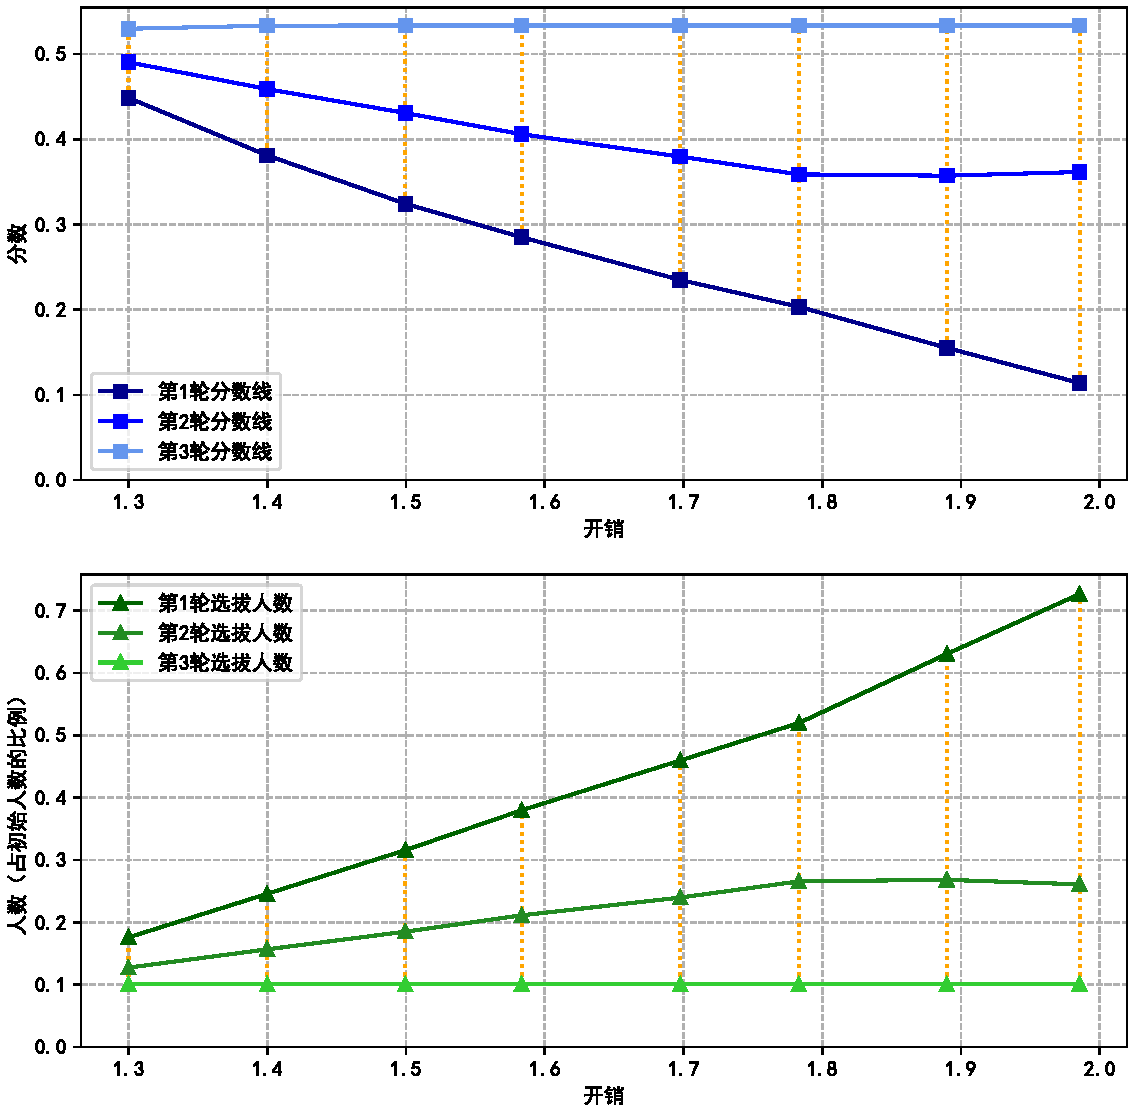
\includegraphics[width=\textwidth]{fig/plottingH1H2H3.pdf}
            \caption{在开销上限的不同取值下,最优解中每一轮次的分数线和人数}
            \label{fig:plottingH1H2H3}
        \end{figure}

        在图\ref{fig:plottingH1H2H3}中,上图展示了所得的每一个最优解中 $h_1,h_2,h_3$ 的取值,下图展示了每一个最优解中分别在 $B_1,B_2,B_3$ 达到分数线的人数(以初始人群大小为单位“1”)。两张图的横轴均表示所得的解的实际开销而非开销上限;由于最优化的过程中存在误差,实际开销并不一定紧贴开销上限。

        \vspace{1.5ex}

        下面以 $T=2.0$ 时的解为例,展示所得选拔过程的选拔效果,见图\ref{fig:plottingOptimizedDistri}。对于 $T$ 的其他取值所绘制的相应图像与图\ref{fig:plottingOptimizedDistri}十分接近,故这里仅展示 $T=2.0$ 时的结果。

        \begin{figure}[htbp]
            \centering
            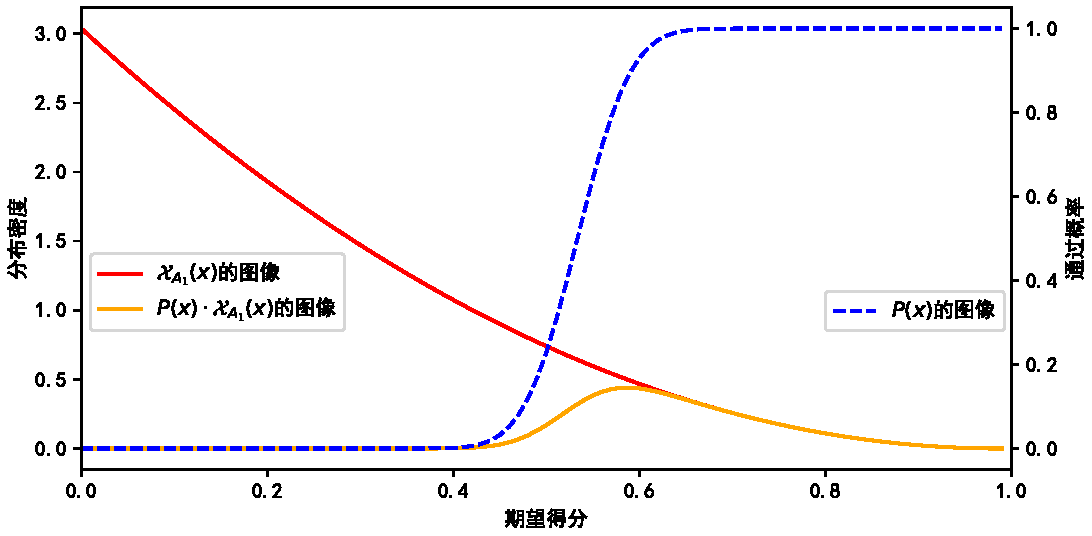
\includegraphics[width=\textwidth]{fig/plottingDistriInOptimizedArrangement.pdf}
            \caption{$T=2.0$时的最优解中,$P(x),\mathcal{X}_{A_1}(x),P(x)\cdot\mathcal{X}_{A_1}(x)$关于$x$的图像}
            \label{fig:plottingOptimizedDistri}
        \end{figure}

\newpage

\section{总结}

    本文建立了描述信息学比赛的数学模型(第\ref{sec:sec2Modeling}节),并基于该模型作出了以下几个发现:
    \begin{itemize}[leftmargin=4em]
        \item 同一名选手的得分波动服从正态分布(第\ref{sec:sec3MeasuringDelta}节)
        \item 联赛复赛的分数分布符合对数曲线(\ref{sec:dataPreprocessingOfNOIP}小节)
        \item 全国信息学选手的水平的分布情况大致符合二次曲线(\ref{sec:calculatingXofSecondRound}小节)
        \item 一名选手按真实水平排序的名次,与该选手在实际比赛中的期望名次、中位名次之间存在特定的关系,且很多时候后两者差于前者(\ref{sec:relationBetweenCapabilityAndRanking}小节)
        \item 在多日比赛中,每日名次与总名次之间存在特定的关系(\ref{sec:relationBetweenEachDayAndTotal}小节)
        \item 在分级选拔中,可以按一定方法设置各级比赛的权重和分数线,以使得选拔效果最好(第\ref{sec:sec6Multilevel}节)
    \end{itemize}

    \vspace{1.5ex}
    
    本文只对信息学竞赛的少数几个方面进行了探究,而即使对于本文着力研究的几个问题,所采用的研究方法在其可靠性、精确性上也有很大改进空间。希望本文能起到抛砖引玉的作用,吸引更多感兴趣的读者来研究有关信息学竞赛本身的问题。

\section{致谢}

    感谢中国计算机学会提供交流和学习的平台;

    感谢国家集训队高闻远教练的指导;

    感谢家人对我的支持和关爱;

    感谢老师、教练们对我的培养;

    感谢清芷等同学与我讨论本文内容。

\begin{thebibliography}{9}
    \bibitem{wiki_sumOfNormVars}
    Wikipedia: Sum of normally distributed random variables,\\
    \inserturl{https://en.wikipedia.org/wiki/Sum\_of\_normally\_distributed\_random\_variables}

    \bibitem{scipy_minimize}
    SciPy Documentation: scipy.optimize.minimize,\\
    \inserturl{https://docs.scipy.org/doc/scipy/reference/generated/scipy.optimize.minimize.html}

    \bibitem{wiki_powerMean}
    Wikipedia: Inequality between any two power means,\\
    \inserturl{https://en.wikipedia.org/wiki/Generalized\_mean\#Inequality\_between\_any\_two\_power\_means}

    \bibitem{scipy_de}
    SciPy Documentation: scipy.optimize.differential\_evolution,\\
    \inserturl{https://docs.scipy.org/doc/scipy/reference/generated/scipy.optimize.differential\_evolution.html}
\end{thebibliography}